\documentclass[../notas medios.tex]{subfiles}
\begin{document}

\chapter{Análisis de Deformaciones}

% Ruta imagenes
\graphicspath{{img/deformaciones/}}

\section{Introducción}
Al final de esta sección el estudiante deberá estar en la capacidad de:

\begin{itemize}
\item[•] Reconocer la diferencia entre desplazamientos absolutos y relativos entre los puntos materiales.
\item[•] Entender los cambios geométricos impartidos al aplicar una transformación lineal sobre un campo vectorial.
\item[•] Identificar los efectos físicos contenidos en el tensor de deformaciones infinitesimales.
\item[•] Calcular el tensor de deformaciones infinitesimales a partir del campo de desplazamientos relativos. 
\item[•] Reconocer la diferencia entre la configuración deformada de un medio continuo y la deformada del punto material
\end{itemize}

Del análisis de las fuerzas ``internas'' se concluyó ---usando las 3 leyes de 
Newton sobre un volumen arbitrario de un medio continuo--- que estas 
corresponden a nivel local a una función (continua) de carácter tensorial y que 
satisface el problema de valores en la frontera especificado por las ecuaciones 
de equilibrio (leyes generalizadas de Newton) y la asignación de las tracciones 
en la superficie del medio (\cref{equtr_5}, \cref{equrot_5}):
\begin{equation} \label{equtr_5}
\begin{split}
& \frac{\partial \sigma_{xx}}{\partial x} + \frac{\partial \tau_{yx}}{\partial y} + \frac{\partial \tau_{zx}}{\partial z} + B_x = 0 \\
& \frac{\partial \tau_{xy}}{\partial x} + \frac{\partial \sigma_{yy}}{\partial y} + \frac{\partial \tau_{zy}}{\partial z} + B_y = 0 \\
& \frac{\partial \tau_{xz}}{\partial x} + \frac{\partial \tau_{yz}}{\partial y} + \frac{\partial \sigma_{zz}}{\partial z} + B_z = 0\, ,
\end{split}
\end{equation}
y
\begin{equation} \label{equrot_5}
\begin{split}
& \tau_{xy} = \tau_{yx} \\
& \tau_{xz} = \tau_{zx} \\
& \tau_{yz} = \tau_{zy}\, .
\end{split}
\end{equation}

Se dispone de 6 ecuaciones en 9 incógnitas controlando la distribución espacial de las fuerzas internas $\sigma$ sobre los diferentes puntos materiales del medio continuo.  Dichas fuerzas internas son generadas por fuerzas de superficie (tracciones) $\vec{t}^{(\hat n)}$  o por interacciones a distancia o fuerzas de cuerpo $\vec {B}$.  Sin embargo, en este punto el problema se hace (matemáticamente) indeterminado ya que se dispone de más incógnitas que ecuaciones.

La indeterminación desde el punto de vista de fuerzas no debe ser para nada sorpresiva, ya que si éstas se consideran como las ``funciones causa'' aún falta involucrar los efectos o ``funciones respuesta". Estas funciones corresponden precisamente a los cambios (cinemáticos) o de configuración, experimentados por las infinitas partículas una vez son sometidas a interacciones externas.

Claramente se identifica la primera necesidad de estudiar los cambios de configuración como la de tratar de establecer una conexión entre estos cambios y las fuerzas internas $\sigma$ y que permita a la postre eliminar la indeterminación matemática del problema de valores en la frontera (PVF) (especificado por las \cref{equtr_5} y \cref{equrot_5}).

Aunque es claro que las nuevas configuraciones aparecen debidas a los desplazamientos a los que son sometidas las diferentes partículas, a la hora de establecer la conexión entre éstas y las fuerzas internas $\sigma$ es importante considerar que son en realidad los desplazamientos relativos  quienes generan estas fuerzas internas.  La aparición de desplazamientos relativos necesariamente se reflejará en términos de cambios de forma  del medio continuo.

\subsection{Concepto intuitivo de deformación}
La \cref{viga1} muestra, en sombreado gris, una viga en voladizo en su configuración original (antes de aplicar las cargas externas) y en línea punteada su configuración final (o deformada)\footnote{En la configuración deformada los puntos materiales o elementos constitutivos de la viga estarán sometidos a un estado de tensiones que satisface las ecuaciones de equilibrio local ( a nivel diferencial) y global.} resultante tras aplicar alguna distribución de cargas externas en forma de tracciones.

Como resultado de la aplicación de las cargas externas los puntos materiales 
que conforman la viga experimentan desplazamientos. En lo que sigue 
denominaremos campo de desplazamientos a la variación espacial de estos, y lo 
denotaremos como $\vec u(\vec x)$. Tal y como se aprecia de manera intuitiva, 
los desplazamientos varían para los diferentes puntos de la viga generándose 
\textbf{desplazamientos relativos}.

\begin{figure}[H]
\centering
	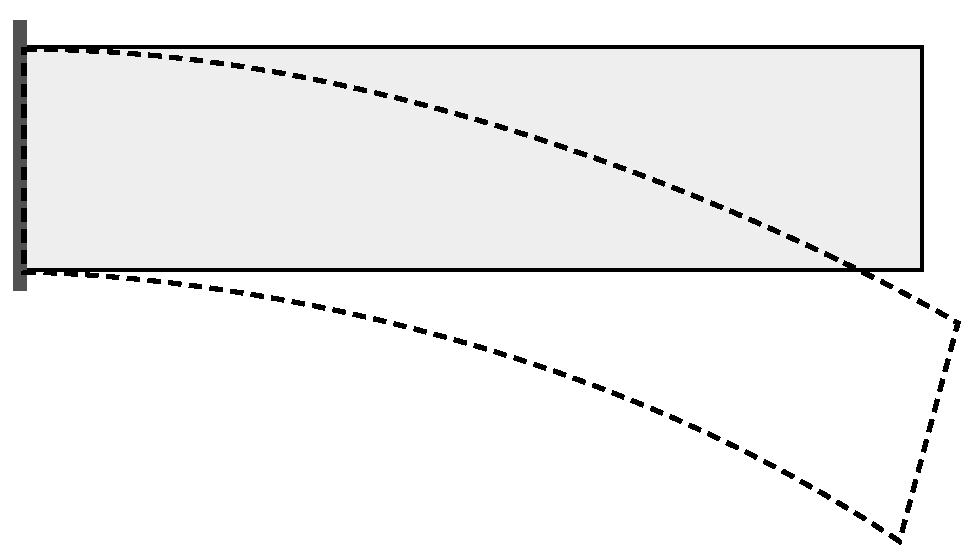
\includegraphics[width=2.5 in]{Fig1.pdf}
	\caption{Configuración original y deformada de una viga en voladizo.}
	\label{viga1}
\end{figure}


Por ejemplo, es evidente que los desplazamientos sobre el empotramiento son "nulos" mientras que los puntos cercanos al extremo derecho de la viga experimentan los máximos desplazamientos. Sin embargo, sabemos que las fuerzas internas (o tensiones) están ligadas al desplazamiento relativo entre los puntos materiales. El propósito de esta sección es hacer una descripción local (o diferencial) de los desplazamientos relativos entre puntos materiales y que pueda ser conectada posteriormente con el tensor de tensiones a través de propiedades de los materiales . Con esto, no solo se conseguirá completar las ecuaciones para el problema de valores en la frontera del medio continuo, sino que además será posible describir la nueva configuración del medio, resultante de la aplicación de interacciones externas tanto a nivel local (diferencial) como global.

Para aclarar, nuevamente de manera intuitiva, el carácter local de los cambios relativos la \cref{steady_state} muestra la configuración original (\cref{nodef}) y deformada (\cref{sidef}) de la viga en voladizo. Como elemento auxiliar de análisis esta vez se ha dibujado una rejilla de elementos perfectamente cuadrados sobre la configuración no-deformada.   Si suponemos que estos elementos son de lado $h$ es claro que en el modelo del continuo el punto material corresponde a uno de estos en el estado limite cuando $h \to 0.$ Es evidente de la \cref{sidef} como los diferentes elementos cambian su forma una vez la viga pasa de la configuración descargada a la cargada. Mas aún es evidente de la misma figura como estos cambios varían de elemento a elemento.

\begin{figure}[H]
     \centering
     \subfloat[Configuración original con elementos diferenciales no deformados]{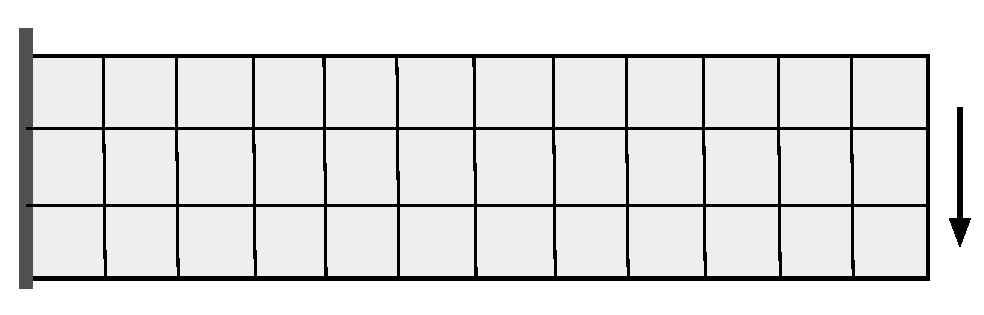
\includegraphics[width=2.8 in]{Fig2a.pdf}\label{nodef}}
     \hspace{0.5cm}\\
     \subfloat[Configuración final con elementos diferenciales deformados]{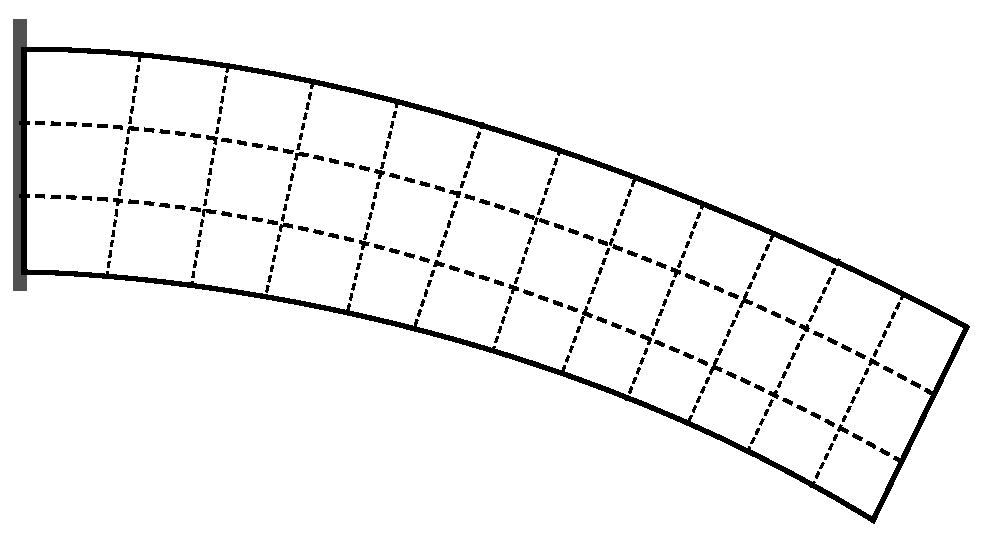
\includegraphics[width=2.8 in]{Fig2b.pdf}\label{sidef}}
     \caption{Comparción entre configuración original y deformada con elementos diferenciales.}
     \label{steady_state}
\end{figure}

La \cref{viga3} muestra nuevamente ambas configuraciones y sobre estas se han 
seleccionado para efectos ilustrativos dos elementos localizados sobre el 
empotramiento y sobre el extremo libre del voladizo. En la configuración 
original ambos elementos son idénticos y corresponden a cuadrados de lado $h$. 
En la configuración deformada, mostrada con líneas punteadas, se resaltan 
nuevamente estos 2 elementos de donde se pueden hacer las siguientes 
observaciones:

El elemento sobre la parte superior del empotramiento experimenta cambios de tamaño y de forma a través de alargamientos en la dirección longitudinal, mientras que el elemento sobre la parte inferior experimenta acortamientos igualmente en la dirección longitudinal. Estos cambios suceden a pesar de que dichos elementos se encuentran sobre el empotramiento donde los desplazamientos como tal son nulos. De otro lado, el elemento sobre el extremo libre de la viga experimenta pequeños cambios de forma  (no apreciables en el dibujo) y experimentan las mayores rotaciones como si fuera un cuerpo rígido. Los pequeños cambios de forma son equivalentes a pequeños desplazamientos relativos aunque estos puntos experimentan los mayores desplazamientos absolutos.


\begin{figure}[H]
\centering
	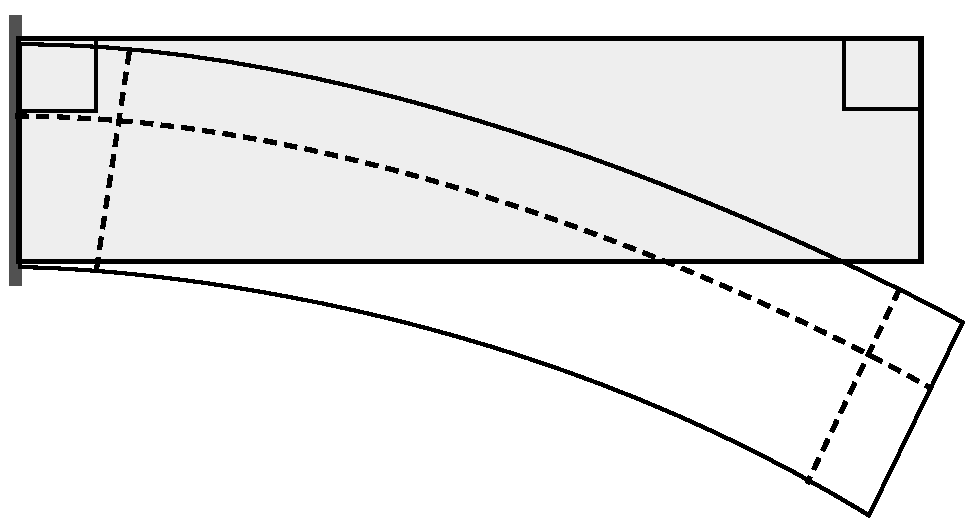
\includegraphics[width=2.5 in]{Fig3.pdf}
	\caption{Elementos con máxima deformación y máxima rotación.}
	\label{viga3}
\end{figure}

En resumen, el propósito de esta sección es hacer una descripción local (o diferencial) de los desplazamientos relativos entre los puntos materiales de un medio continuo cuando este es sometido a la acción de fuerzas externas. En general, como se verá mas adelante, estos cambios se describirán en términos de cambios de tamaño (o magnitud) y de orientación de las "fibras materiales" que emanan de la partícula en las diferentes direcciones tal y como se esquematiza en la \cref{fibras}. Esta muestra un punto material de un medio continuo conjuntamente con su vecindad matemática representada por fibras imaginarias de material, mostradas en líneas punteadas. En la figura el punto material en estudio se muestra con relleno de color negro y se denomina $P$. Adicionalmente se muestra un punto material arbitrario (sin relleno) y denominado $P'$.En el lado izquierdo se muestra la localización de ambos puntos materiales en un instante de tiempo $t=0$, correspondiente a la configuración original o descargada. Tras la aplicación de las cargas ambos puntos materiales se desplazan a las posiciones señaladas como $Q$ y $Q'$ respectivamente y mostradas en lado derecho de la figura correspondiente a un instante de tiempo $t=t$. Como resultado de los desplazamientos experimentados por los puntos materiales la fibra material que une los mismos experimenta cambios de tamaño y de orientación.

\begin{figure}[H]
\centering
	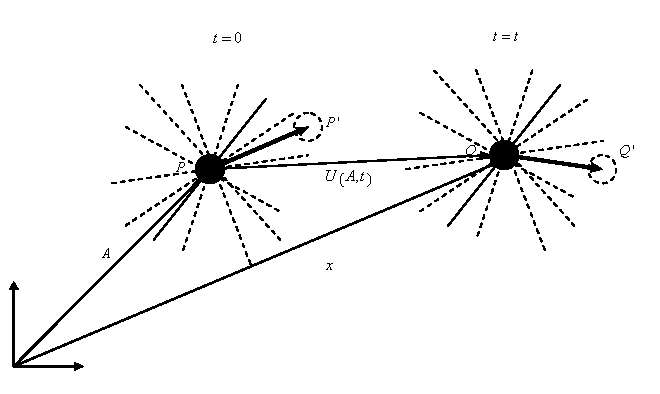
\includegraphics[width=4.0 in]{fibras.pdf}
	\caption{Fibras materiales en la configuración original y deformada.}
	\label{fibras}
\end{figure}

En lo que sigue estudiaremos la relación entre 2 fibras arbitrarias como las mostradas en la figura desde 2 puntos de vista. Inicialmente se estudiarán los cambios de magnitud y orientación experimentados por un vector posición tras operarlo con una matriz conservando la propiedad de línealidad. Posteriormente estudiaremos el problema a nivel infinitesimal tras analizar un par de puntos, unidos por una fibra material de tamaño diferenial. Dicho analisis permitirá encontrar el tensor graiente de desplazamientos como medida local (o diferencial) de la deformación\footnote{Aunque hasta el momento el tratamiento del medio continuo no ha especificado ninguna diferencia entre medios sólidos, liquidos o gases el tratamiento cinematico que se presenta si esta restringido al caso de pequeñas deformaciones}.


\section{Transformaciones lineales}
Con el propósito de conceptualizar el proceso deformación o cambios de configuración a nivel local o diferencial es conveniente apoyarnos como herramienta de análisis en las transformaciones lineales\footnote{Esta sección esta basada en los textos: Principles of Solid Mechanics. Rowland Richards Jr. CRC Press, 2001 y Introduction to the Mechanics of Continuous Medium. Lawrence E Malvern. Prentice Hall, 1969.}. En términos simples estas corresponden a la traformación de un vector en otro conservando la propiedad de línealidad. Esta idea se ilustra en la \cref{amat} en la que $\vec r = {r_x}\hat i + {r_y}\hat j$ representa el vector posición de un punto $P$. Como resultado de alguna acción externa, representada por un tensor $A$ este punto material experimenta un desplazamiento $\vec \Delta  = {\Delta _x}\hat i + {\Delta _y}\hat j$ con lo que que el vector $\vec{r}$ se transforma en el vector $\vec \rho  = {\rho _x}\hat i + {\rho _y}\hat j$. Esta relación puede escribirse como:
\begin{equation}
\vec \rho  = A \cdot \vec r
\label{amat}
\end{equation}

\begin{figure}[H]
\centering
	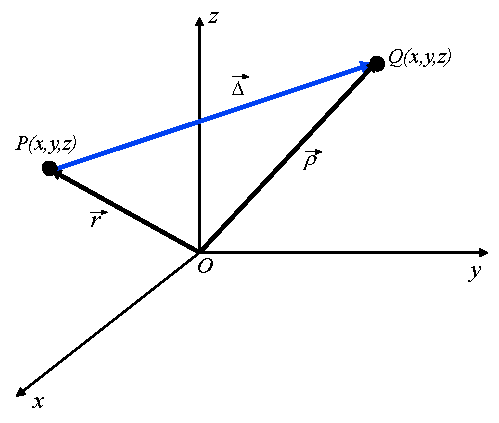
\includegraphics[width=3.0 in]{trans.pdf}
	\caption{Transformación del vector $\vec{r}$ en el vector $\vec{\rho}$.}
	\label{trans}
\end{figure}

El vector $\vec{r}$ al transformarse en el vector $\vec{\rho}$ experimenta 2 tipos de cambios:
\begin{itemize}
\item[i] Cambios de magnitud (o de tamaño).
\item[ii] Cambios de orientación (dirección). 
\end{itemize}

La relación \cref{amat} entre $\vec{r}$ y $\vec{\rho}$ puede escribirse en forma explicita como:
\begin{equation}
\left\{ {\begin{array}{*{20}{c}}
{{\rho _x}}\\
{{\rho _y}}
\end{array}} \right\} = \left[ {\begin{array}{*{20}{c}}
{{a_{xx}}}&{{a_{xy}}}\\
{{a_{yx}}}&{{a_{yy}}}
\end{array}} \right]\left\{ {\begin{array}{*{20}{c}}
{{r_x}}\\
{{r_y}}
\end{array}} \right\}
\label{roaere}
\end{equation}

La \cref{roaere} indica que la matriz $A$ transforma el vector $\vec{r}$ en el vector $\vec{\rho}$ y por ende ésta contiene toda la información referente a los cambios de magnitud y dirección que experimentan las infinitas direcciones que emanan del punto $O$. Una transformación como la descrita en la \cref{roaere} se denomina lineal si satisface la condición dada por:
\begin{equation}
A \cdot (\vec{r}_1 + \vec{r}_2) = A \cdot \vec{r}_1 + A \cdot \vec{r}_2
\label{lineal}
\end{equation}

la cual implica que lineas rectas y paralelas antes de la transformación permanecen rectas y paralelas después de la transformación o en otras palabras que conservan la ley del paralelogramo. Esto se ilustra en la \cref{paralelo}:
\begin{figure}[H]
\centering
	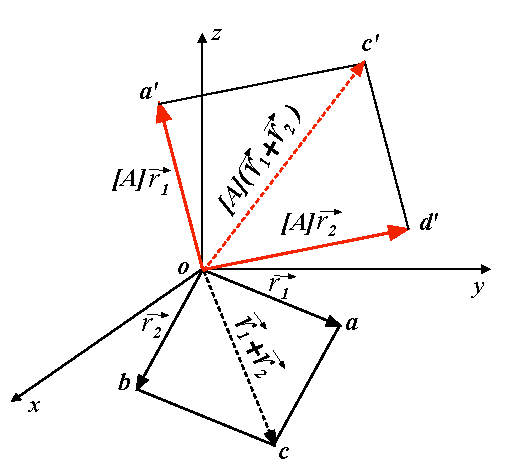
\includegraphics[width=3.0 in]{paralelo.pdf}
	\caption{Definición de linealidad.}
	\label{paralelo}
\end{figure}

Alternativamente, es posible escribir la transformación en términos del vector 
de desplazamientos $\vec {\Delta}$  que experimenta la cabeza del vector 
$\vec{r}$ como sigue:  
\begin{align*}
&\vec \Delta  = \vec \rho  - \vec r\\
&\vec \Delta  = A \cdot \vec r - \vec r\\
&\vec \rho  = \left[ {A - I} \right] \cdot \vec r\\
&\vec \Delta  = D \cdot \vec r
\end{align*}
y de manera explícita escribimos
\begin{equation}
\begin{Bmatrix}
\Delta_x\\
\Delta_y
\end{Bmatrix}= 
\begin{bmatrix}
d_{xx} &d_{xy}\\
d_{yx} &d_{yy}
\end{bmatrix}
\begin{bmatrix}
r_x\\
r_y
\end{bmatrix}
\label{disp}
\end{equation}

La matriz $D$ se denomina la matriz de transformación de desplazamientos. En lo que sigue estudiaremos transformaciones como las dadas en la \cref{disp} identificando los efectos que dicha matriz impone sobre las diferentes direcciones que emanan de un punto material. 

\subsection{Componente rotacional}
A continuación nos disponemos a estudiar el efecto de los diferentes términos en la matriz de transformación de desplazamientos $D$. Abordemos inicialmente los cambios de orientación impartidos por $D$ en los diferentes vectores. Considerando la \cref{rota}, en esta el vector original $\vec{r}$ se transforma en el vector $\rho$ tras realizar una rotación $\alpha$. 

\begin{figure}[H]
\centering
	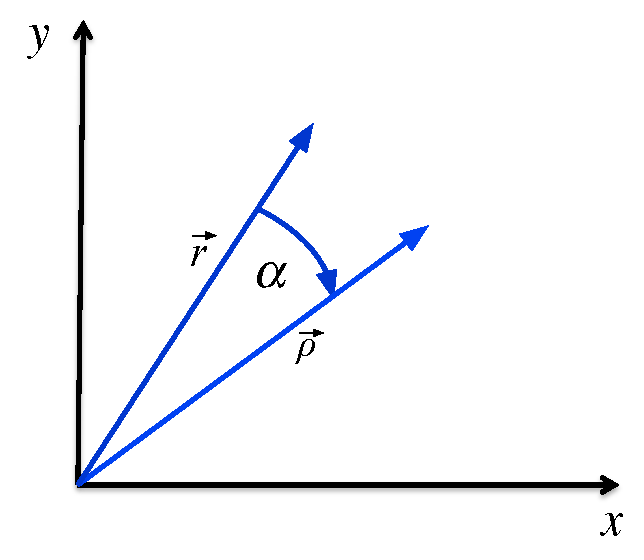
\includegraphics[width=3.0 in]{rota.pdf}
	\caption{Rotación a través de un ángulo $\alpha$ del vector $\vec{r}$ en el 
	vector $\vec{\rho}$.}
	\label{rota}
\end{figure}


Relacionando las componentes rectangulares de ambos vectores se tiene que:
\[\rho_x = r_x + \alpha r_y\]
y
\[\rho_y = r_y - \alpha r_x\, .\]

De manera explicita, pero en términos de los desplazamientos de la cabeza del vector posición $\vec{r}$ lo anterior resulta en:

\begin{equation}
\begin{Bmatrix}
\Delta_x\\
\Delta_y
\end{Bmatrix}=
\begin{bmatrix}
0 &\alpha \\
-\alpha &0
\end{bmatrix}
\begin{Bmatrix}
r_x\\
r_y
\end{Bmatrix}
\label{asym}
\end{equation}

De la \cref{asym} se concluye que la componente rotacional del tensor de 
transformación de desplazamientos $D$ es una matriz con ceros en la diagonal y 
términos iguales pero con signo opuesto a uno y otro lado de la diagonal. En el 
lenguaje del análisis tensorial, extendido en este caso a matrices, a estos 
tensores se les conoce como tensores anti-simétricos. En conclusión \emph{la 
componente rotacional de la transformación lineal corresponde a un tensor 
anti-simétrico.}


\subsection{Componente simétrica}
Como ya ha sido identificado en los planteamientos anteriores, la matriz de 
transformación de desplazamientos $D$ imparte en las diferentes direcciones 
cambios de dirección y de magnitud. El haber identificado el efecto rotacional 
como la componente anti-simétrica de $D$ permite concluir que el término 
restante, y simétrico por demás, contendrá los efectos asociados a los cambios 
de tamaño o magnitud de los diferentes vectores. De dicha conclusión resulta 
natural resolver el tensor $D$ precisamente en una componente simétrica y en 
una componente anti-simétrica como:
\begin{equation}
\begin{bmatrix}
d_{xx} &d_{xy}\\
d_{yx} &d_{yy}
\end{bmatrix} = \begin{bmatrix}
d_{xx} &\frac{d_{xy} + d_{yx}}{2}\\
\frac{d_{yx} + d_{xy}}{2} &d_{yy}
\end{bmatrix} + \begin{bmatrix}
0 &\frac{d_{xy} - d_{yx}}{2}\\
\frac{d_{yx} - d_{xy}}{2} &0
\end{bmatrix}\, .
\label{descomp}
\end{equation}

En esta partición es evidente que el segundo término del lado derecho 
corresponde efectivamente a la componente rotacional del tensor (componente 
anti-simétrica), mientras que el primer término necesariamente contendrá la 
información relativa a los cambios de tamaño. Nótese además que este primer 
término es simétrico con respecto a la diagonal. De forma general escribimos 
esta partición de la matriz de transformación de desplazamientos $D$ como:
\begin{equation}
D = \varepsilon  + \omega
\label{parti}
\end{equation}
donde $\varepsilon$ contiene los efectos de cambio de tamaño y $\omega$ contiene los efectos de cambio de orientación.

Para estudiar los efectos de las diferentes componentes del tensor de transformación de desplazamientos $D$ usaremos el cuadrado unitario de la \cref{unitario}.

\begin{figure}[H]
\centering
	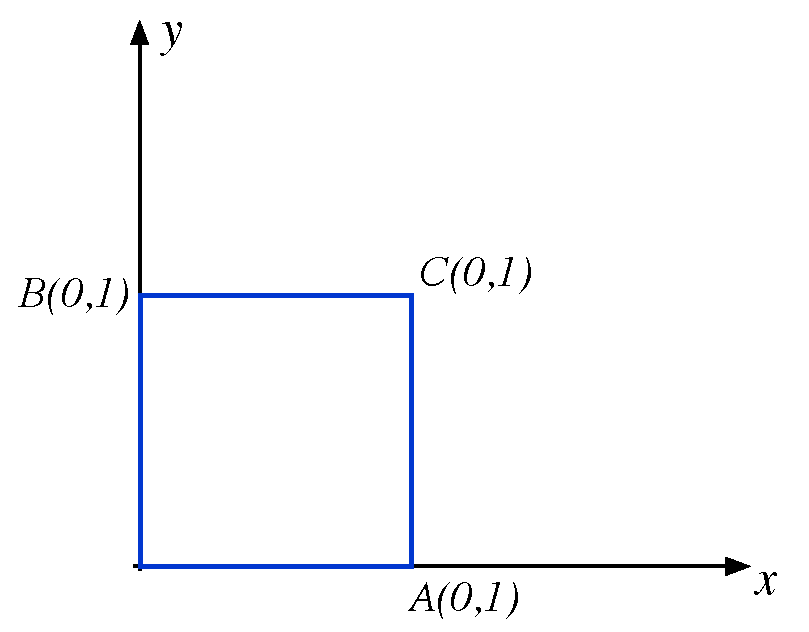
\includegraphics[width=2.0 in]{unitario.pdf}
	\caption{Cuadrado unitario a ser transformado por el tensor $D$.}
	\label{unitario}
\end{figure}

Como método de análisis aplicaremos las diferentes componentes del tensor $D$ 
sobre los vectores posición de los puntos $A$, $B$ y $C$ dados por:
\[{{\vec r}_A} = 1.0\hat i\]
\[{{\vec r}_B} = 1.0\hat j\]
\[{{\vec r}_C} = 1.0\hat i + 1.0\hat j\]
y asumiremos que los puntos $O$, $A$, $B$ y $C$ permanecen unidos por líneas rectas de acuerdo con la propiedad de linealidad. Posteriormente compararemos la configuración original y deformada del elemento.

Consideremos inicialmente la componente simétrica de la \cref{parti}. Por 
razones que se harán evidentes más adelante denotemos los elementos de esta 
componente como:
\[\varepsilon  = \begin{bmatrix}
\varepsilon_{xx} &\bar{\gamma} \\
\bar{\gamma} &\varepsilon_{yy}
\end{bmatrix}\]

Para determinar la configuración deformada aplicamos la expresión:
\[\begin{Bmatrix}
\Delta x\\
\Delta y
\end{Bmatrix} = \begin{bmatrix}
\varepsilon_{xx} &\bar{\gamma} \\
\bar{\gamma} & \varepsilon_{yy}
\end{bmatrix} \begin{Bmatrix}
r_x\\
r_y
\end{Bmatrix}\]
a los vectores posición $\vec{r}_A$, $\vec{r}_B$ y $\vec{r}_C$. Esto da como 
resultado los vectores de desplazamiento:
\begin{align*}
&\vec{\Delta}_A = \varepsilon_{xx} \hat \imath + \bar{\gamma} \hat \jmath\\
&\vec{\Delta}_B = \bar{\gamma} \hat \imath + \varepsilon_{yy}\hat \jmath\\
&\vec{\Delta}_C = (\varepsilon_{xx} + \bar{\gamma})\hat \imath + 
(\varepsilon_{yy} + \bar{\gamma} )\hat \jmath
\end{align*}
y la configuración deformada mostrada en línea punteada en la \cref{sime}.

\begin{figure}[H]
\centering
	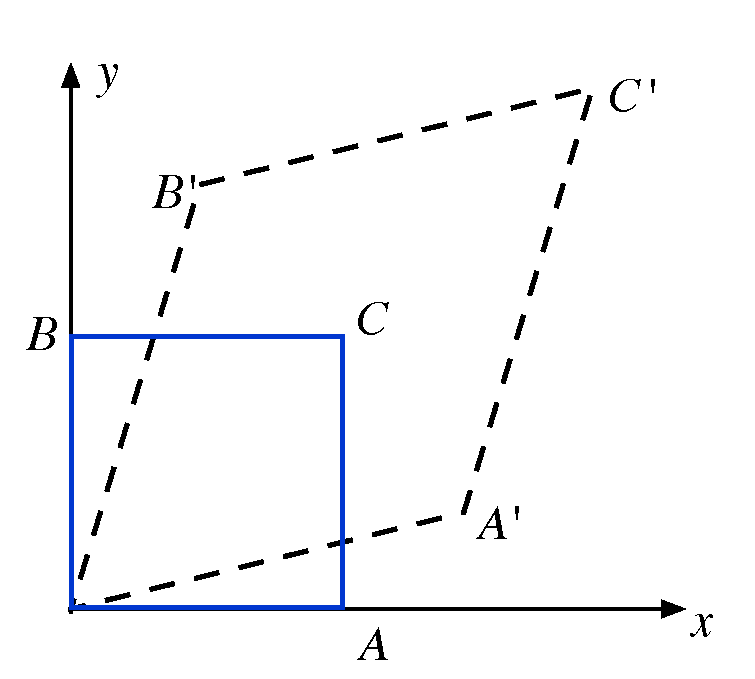
\includegraphics[width=2.5 in]{simetrica.pdf}
	\caption{Configuraciones original y deformada de un cuadrado unitario debido a la componente simétrica $\varepsilon$ del tensor de transformación de desplazamientos $D$.}
	\label{sime}
\end{figure}

\subsection{Componentes escalar y distorsional}
La componente simétrica del tensor de transformación de desplazamientos es 
análoga al tensor de tensiones estudiado en secciones anteriores. De hecho, 
dado su carácter simétrico este puede ser estudiado en términos del circulo de 
Mohr. Identificando esta conexión es posible resolver esta componente en 
términos adicionales que permiten ahondar en el entendimiento físico del 
análisis de deformaciones. En particular considere la siguiente descomposición:
\begin{equation}
\begin{bmatrix}
\varepsilon_{xx} &\bar{\gamma} \\
\bar{\gamma} &\varepsilon_{yy}
\end{bmatrix} = \begin{bmatrix}
\frac{\varepsilon_{xx} + \varepsilon_{yy}}{2} &0\\
0 &\frac{\varepsilon_{xx} + \varepsilon_{yy}}{2}
\end{bmatrix} + \begin{bmatrix}
\frac{\varepsilon_{xx} - \varepsilon_{yy}}{2} &0\\
0 &\frac{\varepsilon_{yy} - \varepsilon_{xx}}{2}
\end{bmatrix} + \begin{bmatrix}
0 &\bar{\gamma} \\
\bar{\gamma} &0
\end{bmatrix}
\label{otras}
\end{equation}
en la cual se ha separado la componente simétrica en un término escalar 
(correspondiente al centro del círculo de Mohr) y en 2 términos con información 
distorsional controlando el radio del círculo. Escribamos la descomposición de 
$\varepsilon$ como:
\[\varepsilon  = pI + S + C\]
donde se reconoce $p=\frac{\varepsilon_{xx} + \varepsilon_{yy}}{2}$ 
con lo que el primer término se escribe como:
\[pI = \begin{bmatrix}
\frac{\varepsilon_{xx} + \varepsilon_{yy}}{2} &0\\
0 &\frac{\varepsilon_{xx} + \varepsilon_{yy}}{2}
\end{bmatrix}\, .\]

Similarmente, haciendo $s = \frac{\varepsilon_{xx} - \varepsilon_{yy}}{2}$ 
escribimos:
\[S = \begin{bmatrix}
\frac{\varepsilon_{xx} - \varepsilon_{yy}}{2} &0\\
0 &\frac{\varepsilon_{yy} - \varepsilon_{xx}}{2}
\end{bmatrix} \equiv \begin{bmatrix}
s &0\\
0 &-s
\end{bmatrix}\]
y finalmente
\[C = \begin{bmatrix}
0 &\bar{\gamma} \\
\bar{\gamma} &0
\end{bmatrix}\, .\]

Para entender el efecto físico de cada uno de estos términos aplicaremos nuevamente la transformación al cuadrado unitario previamente definido.

La componente escalar $pI$ genera los siguientes vectores de desplazamientos 
tras aplicar la \cref{disp}:
\begin{align*}
&\vec{\Delta}_A = p\hat \imath\\
&\vec{\Delta}_B = p\hat \jmath\\
&\vec{\Delta}_C = p\hat \imath + p\hat \jmath
\end{align*}
resultando en el cambio de forma mostrado en la \cref{scalar}

\begin{figure}[H]
\centering
	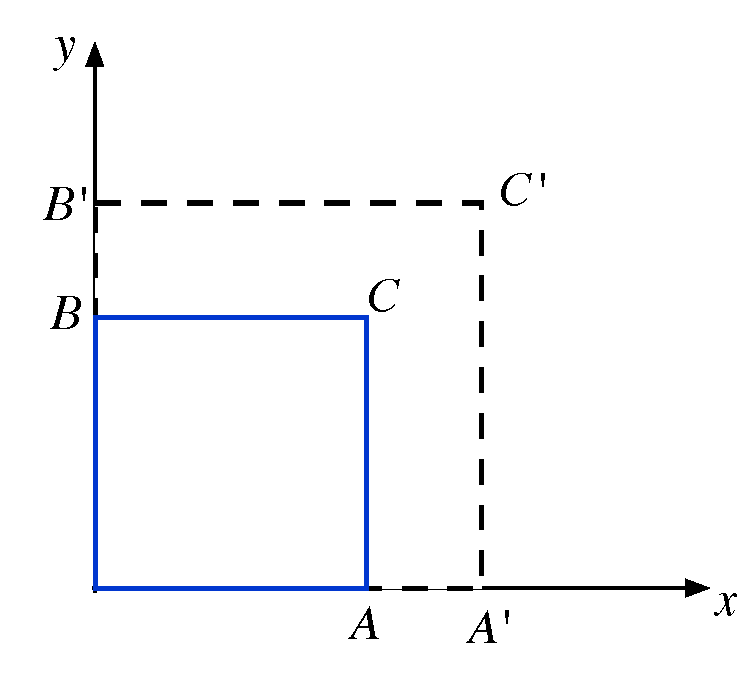
\includegraphics[width=2.5 in]{scala.pdf}
	\caption{Configuraciones original y deformada de un cuadrado unitario debido a la componente escalar de la componente simétrica del tensor de transformación de desplazamientos.}
	\label{escalar}
\end{figure}

De manera similar, la primera componente distorsional $S$ genera los siguientes 
vectores de desplazamientos:
\begin{align*}
&\vec{\Delta}_A = s\hat \imath\\
&\vec{\Delta}_B =  - s\hat \jmath\\
&\vec{\Delta}_C = s\hat \imath - s\hat \jmath
\end{align*}
resultando en el cambio de forma mostrado en la \cref{disto1}.

\begin{figure}[H]
\centering
	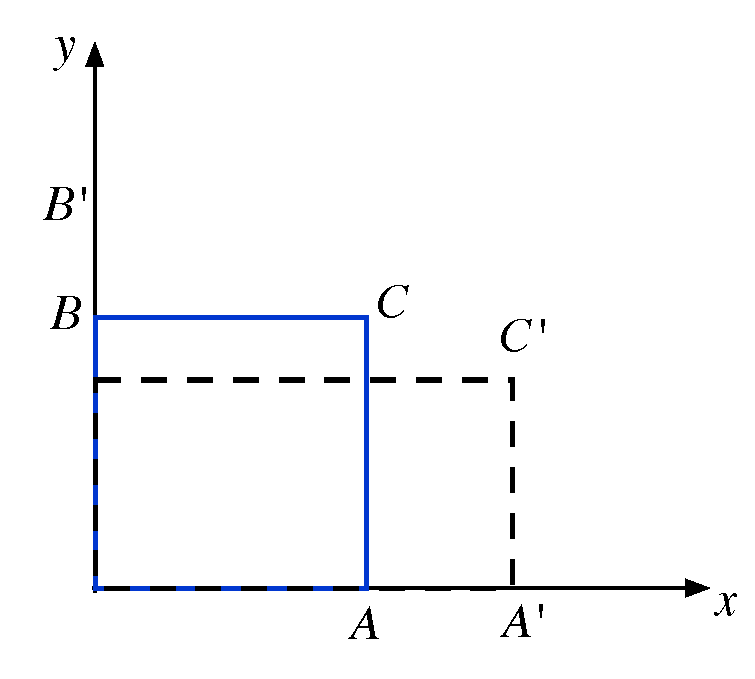
\includegraphics[width=2.5 in]{disto1.pdf}
	\caption{Configuraciones original y deformada de un cuadrado unitario debido a la primera componente distorsional de la componente simétrica del tensor de transformación de desplazamientos.}
	\label{disto1}
\end{figure}

Luego, aplicando la segunda componente distrosional $C$ da como resultado los siguientes vectores de desplazamientos:
\begin{align*}
&\vec{\Delta}_A = \gamma \hat \jmath\\
&\vec{\Delta}_B = \gamma \hat \imath\\
&\vec{\Delta}_C = \gamma \hat \imath + \gamma \hat \jmath
\end{align*}
y en los cambios de configuración mostrados en la \cref{disto2}
\begin{figure}[H]
\centering
	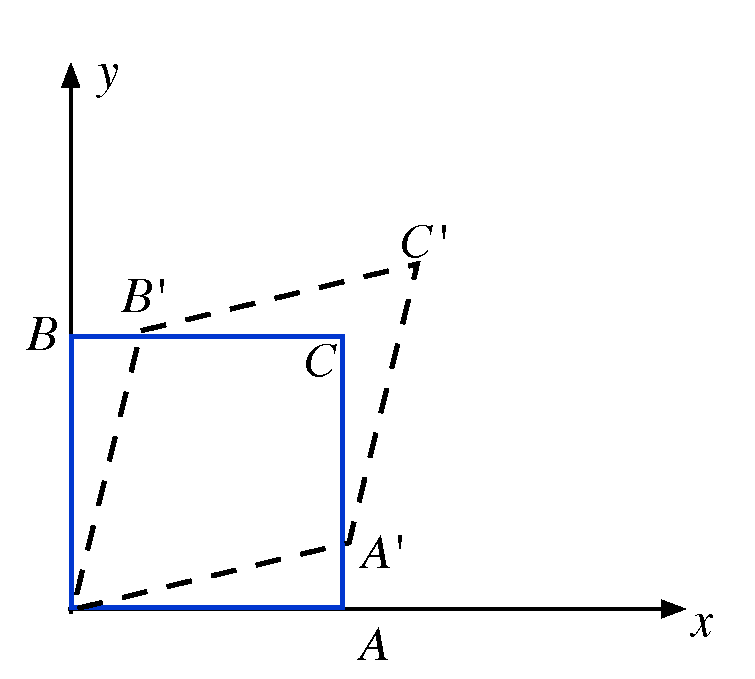
\includegraphics[width=2.5 in]{disto2.pdf}
	\caption{Configuraciones original y deformada de un cuadrado unitario debido a la segunda componente distorsional de la componente simétrica del tensor de transformación de desplazamientos.}
	\label{disto2}
\end{figure}

Finalmente, y en aras de la consistencia apliquemos la componente rotacional 
$\omega$ (ver \cref{parti}) al cuadrado unitario obteniendo como resultado los 
siguientes vectores de desplazamiento:
\begin{align*}
&\vec{\Delta}_A =  - \alpha \hat \jmath\\
&\vec{\Delta}_B = \alpha \hat \imath\\
&\vec{\Delta}_C = \alpha \hat \imath - \alpha \hat \jmath
\end{align*}
y el cambio de configuración mostrado en la \cref{rotarota}

\begin{figure}[H]
\centering
	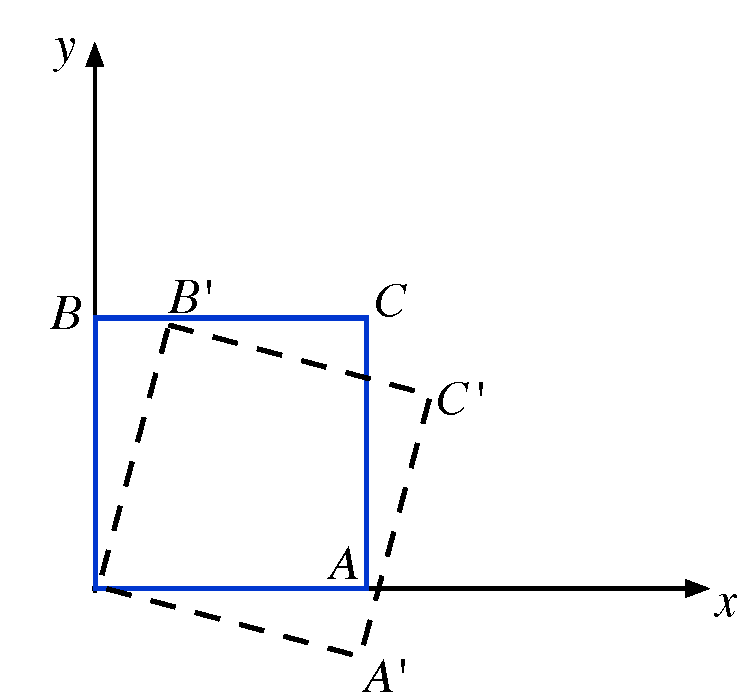
\includegraphics[width=2.5 in]{omega.pdf}
	\caption{Configuraciones original y deformada de un cuadrado unitario debido a la componente anti-simétrica del tensor de transformación de desplazamientos.}
	\label{rotarota}
\end{figure}


\subsection*{Ejemplo}
Un tensor dado $D$ permite calcular los desplazamientos $\Delta$   de los 
puntos en un espacio (en 2-dimensiones) y cuya posición original se encuentra 
dada por el vector posición ${\vec r}$   de acuerdo con
\[\vec \Delta  = D \cdot \vec r\, .\]

El este tensor resulta de superponer (o sumar) los 2 efectos mostrados en la \cref{eje1a} y \cref{eje1b} en la cual las líneas continuas representan la configuración original y las líneas punteadas la configuración final.

\begin{figure}[H]
     \centering
     \subfloat[Cambios debidos a la componente simétrica]{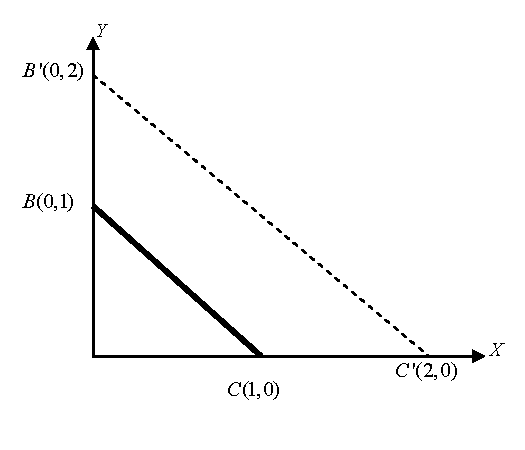
\includegraphics[width=2.8 in]{eje1a.pdf}\label{eje1a}}
     \hspace{0.5cm}
     \subfloat[Cambios debidos a la componente anti-simétrica]{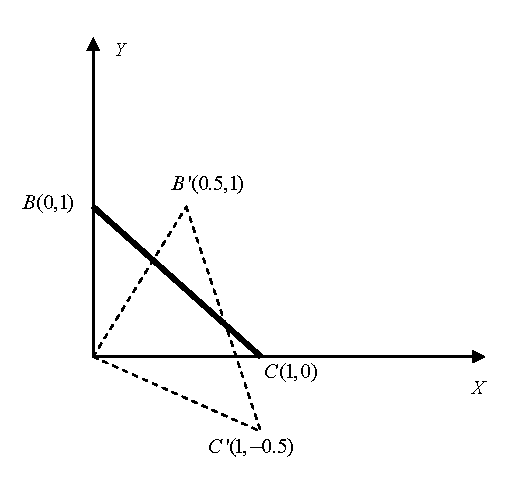
\includegraphics[width=2.8 in]{eje1b.pdf}\label{eje1b}}
     \caption{Transformación líneal de elemento triangular.}
     \label{steady_state1}
\end{figure}

Se pide:

\begin{itemize}
\item (i) Determinar el tensor $D$.
\item (ii) Determinar las componentes simétrica $\varepsilon$ y anti-simétrica $\omega$ del tensor $D$.
\item (iii) Determinar las direcciones y valores principales de la componente simétrica $\varepsilon$.
\end{itemize}

En la primera transformación se tienen los siguientes vectores de posición 
originales
\begin{align*}
&\vec{r}_B = 1.0\hat \jmath\\
&\vec{r}_C = 1.0\hat \imath
\end{align*}
y los siguientes vectores de desplazamientos para los puntos $B$ y $C$ 
respectivamente;
\begin{align*}
&\vec \Delta_B = 1.0\hat \jmath\\
&\vec \Delta_C = 1.0\hat \imath
\end{align*}
planteando para cada punto la ecuación:
\[\begin{Bmatrix}
\Delta_x\\
\Delta_y
\end{Bmatrix} = \begin{bmatrix}
\varepsilon_{xx} &\bar{\gamma} \\
\bar{\gamma} &\varepsilon_{yy}
\end{bmatrix}\begin{Bmatrix}
r_x\\
r_y
\end{Bmatrix}\]
permite determinar;
\[\varepsilon \equiv \begin{bmatrix}
\varepsilon_{xx} &\bar{\gamma}\\
\bar{\gamma} &\varepsilon_{yy}
\end{bmatrix} = \begin{bmatrix}
1.0 &0.0\\
0.0 &1.0
\end{bmatrix}\, .\]

De manera análoga, en el caso de la segunda transformación se tiene que
\[\omega  \equiv \begin{bmatrix}
0 &\alpha \\
-\alpha &0
\end{bmatrix} = \begin{bmatrix}
0.0 &0.5\\
-0.5 &0.0
\end{bmatrix}\]
por lo que el tensor resultante corresponde a:
\[\varepsilon  + \omega  \equiv \begin{bmatrix}
1.0 &0.0\\
0.0 &1.0
\end{bmatrix} + \begin{bmatrix}
0.0 &0.5\\
-0.5 &0.0
\end{bmatrix} \equiv \begin{bmatrix}
1.0 &0.5\\
-0.5 &1.0
\end{bmatrix}\, .\]

\subsection*{Problema propuesto}

La \cref{problem} corresponde a la configuración original de un medio continuo. Si sobre este se aplica el tensor de transformación de desplazamientos:
\[D = \begin{bmatrix}
d_{xx} &d_{xy}\\
d_{yx} &d_{yy}
\end{bmatrix}\]
determinar la configuración deformada del medio indicando claramente el efecto 
de cada una de las componentes definidas de acuerdo con:
\[D = \varepsilon  + \omega  \equiv pI + S + C + \omega \]
\begin{figure}[H]
\centering
	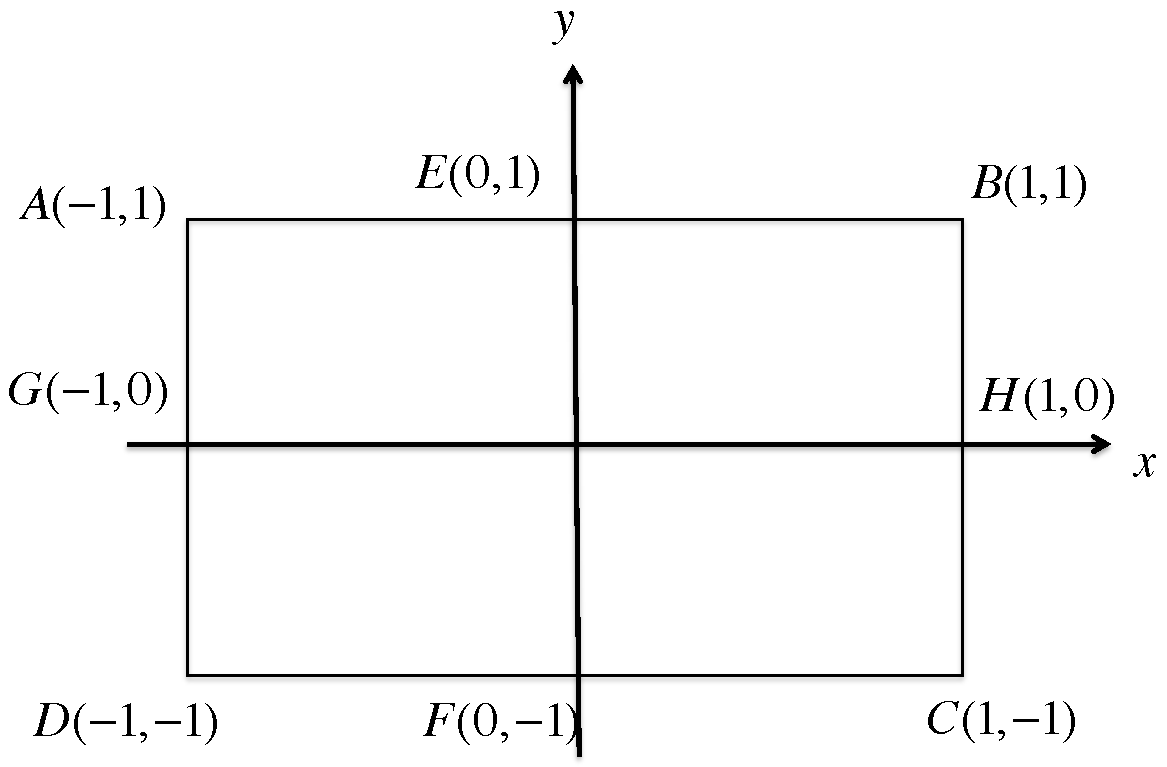
\includegraphics[width=3.5 in]{problemCap5.pdf}
	\caption{Transformación al espacio completo.}
	\label{problem}
\end{figure}


\section{Tensor de deformaciones unitarias}
Procedamos ahora a comparar lo que sucede con una fibra materiales 
infinitesimal tras haber sido sometida al proceso de deformación. Ésta se 
muestra en la \cref{pelos} conectando los puntos materiales que ocupan las 
posiciones $P$ y $Q$ antes de la deformación y las posiciones $p$ y $q$ en la 
configuración deformada. En la configuración original la fibra $PQ$ esta dada 
por el vector $d\vec{r}$ expresado en términos de magnitud y dirección como:
\[\dd{\vec r} = \hat n\dd{S}\]
donde
\[\hat n = \dv{x}{S}\hat \imath + \dv{y}{S}\hat \jmath\, .\]

\begin{figure}[H]
\centering
	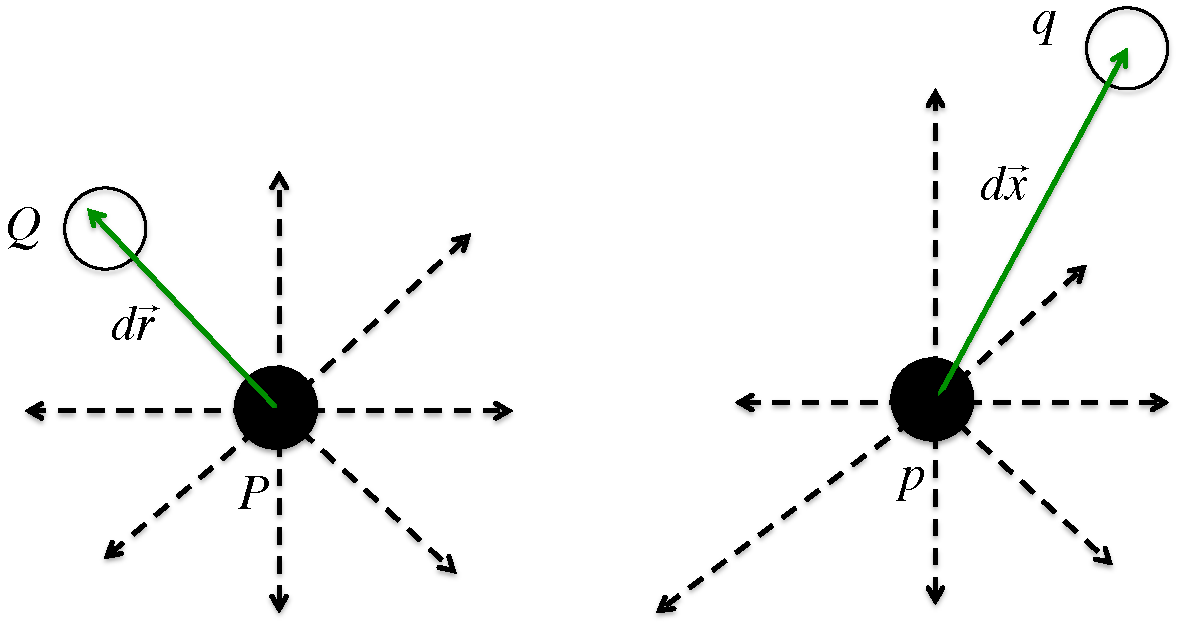
\includegraphics[width=4.0 in]{pelos.pdf}
	\caption{Fibras materiales emanando de un punto material $P$ en las configuraciones original y deformada.}
	\label{pelos}
\end{figure}

En la configuración deformada la fibra $PQ$ se convierte en la fibra $pq$ dada 
por el vector $d\vec{x}$. Ambas se comparan en la \cref{relative} en la que 
también se identifica el desplazamiento $\vec{u}_P$ del punto material $P$ y el 
desplazamiento $\vec{u}_Q$  del punto material $Q$.

\begin{figure}[H]
\centering
	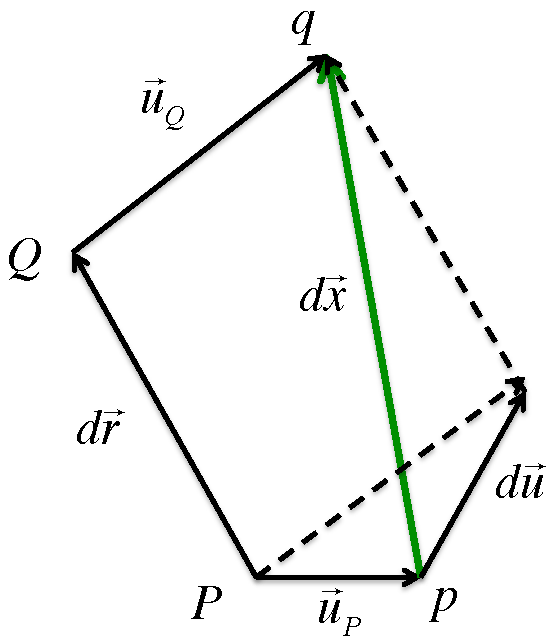
\includegraphics[width=2.5 in]{relative.pdf}
	\caption{Desplazamiento relativo entre 2 puntos materiales infinitesimalmente cercanos.}
	\label{relative}
\end{figure}

Escribiendo el desplazamiento relativo $\dd{\vec u}$  en términos de los 
vectores fibra original y deformado $\dd{\vec{r}}$ y $\dd{\vec{x}}$  se tiene:
\[\dd{\vec u} = \dd{\vec x} - \dd{\vec r}\]
o usando una relación como:
\[\dd{\vec x} = A \cdot \dd{\vec r}\]
donde $A$ transforma $\dd{\vec{r}}$ en $\dd{\vec{x}}$ se tiene:
\[\dd{\vec u} = [A - I] \cdot \dd{\vec r}\]
o, finalmente,
\begin{equation}
\dd{\vec u} = J \cdot \dd{\vec r}.
\label{jacobian}
\end{equation}

En la expresión \cref{jacobian} el tensor $J$ \footnote{El tensor $J$ es el 
análogo al tensor $D$ visto en la sección de trasformaciones lineales} permite 
obtener el desplazamiento relativo $d\vec{u}$ del punto material $Q$ con 
respecto a $P$. Escribiendo $d\vec{u}$ en términos de sus componentes 
rectangulares como
\[\dd{\vec u} = \dd{u}\hat \imath + \dd{v}\hat \jmath\]
permite escribir la \cref{jacobian} en forma explicita de acuerdo con:
\[\begin{Bmatrix}
\dd{u}\\
\dd{v}
\end{Bmatrix} = \begin{bmatrix}
J_{xx} &J_{xy}\\
J_{yx} &J_{yy}
\end{bmatrix}\begin{Bmatrix}
\dd{x}\\
\dd{y}
\end{Bmatrix}\, .\]

Reconociendo los términos del tensor $J$ como las variaciones de las 
componentes rectangulares $\dd{u}$ y $\dd{v}$ a lo largo de distancias 
diferenciales $\dd{x}$ y $\dd{y}$ permite escribir:
\begin{align*}
&\dd{u} = J_{xx} \dd{x} + J_{xy}\dd{y} \equiv \pdv{u}{x}\dd{x} + 
\pdv{u}{y}\dd{y}\\
&\dd{v} = J_{yx}\dd{x} + J_{yy}\dd{y} \equiv \pdv{v}{x}\dd{x} + 
\pdv{v}{x}\dd{y}
\end{align*}
o en forma explicita:
\[\begin{Bmatrix}
\dd{u}\\
\dd{v}
\end{Bmatrix} = \begin{bmatrix}[1.5]
\pdv{u}{x} &\pdv{u}{y}\\
\pdv{v}{x} &\pdv{v}{y}
\end{bmatrix}\begin{Bmatrix}
\dd{x}\\
\dd{y}
\end{Bmatrix}\]
y en donde el tensor $J$ corresponde al gradiente de desplazamientos. 
Normalizando el vector de desplazamientos relativos por la magnitud original 
$\dd{S}$ de la fibra, permite obtener el desplazamiento relativo unitario como 
una transformación
\[\begin{Bmatrix}[1.5]
\dv{u}{S}\\
\dv{v}{S}
\end{Bmatrix} = \begin{bmatrix}[1.5]
\pdv{u}{x} &\pdv{u}{y}\\
\pdv{v}{x} &\pdv{v}{y}
\end{bmatrix} \begin{Bmatrix}[1.5]
\dv{x}{S}\\
\dv{y}{S}
\end{Bmatrix}\]
o
\begin{equation}
\left\{\dv{\vec u}{S}\right\}  = J \cdot \hat n.
\label{trans}
\end{equation}

Para identificar los diferentes efectos contenidos en el gradiente de 
desplazamientos este se descompone en términos de sus componentes simétrica y 
anti-simétrica como:
\[J = \varepsilon  + \omega \]
o en forma explicita:
\[\begin{bmatrix}[1.5]
\pdv{u}{x} &\pdv{u}{y}\\
\pdv{v}{x} &\pdv{v}{y}
\end{bmatrix} = \begin{bmatrix}[1.5]
\pdv{u}{x} &\frac{1}{2}\left(\pdv{u}{y} + \pdv{v}{x}\right)\\
\frac{1}{2}\left(\pdv{u}{y} + \pdv{v}{x}\right) &\pdv{v}{y}
\end{bmatrix} + \begin{bmatrix}[1.5]
0 &\frac{1}{2}\left(\pdv{u}{y} - \pdv{v}{x}\right)\\
-\frac{1}{2}\left(\pdv{u}{y} - \pdv{v}{x}\right) &0
\end{bmatrix}\]

Los efectos físicos de las diferentes componentes del tensor $J$ serán estudiados analizando los cambios impuestos por este sobre el elemento diferencial mostrado en la \cref{diferencial}. En particular, se calcularán los desplazamientos de los puntos $A$, $B$ y $C$ con vectores posición:
\begin{align*}
\vec{r}_A = \dd{x}\hat \imath\\
\vec{r}_B = \dd{y}\hat \jmath\\
\vec{r}_C = \dd{y}\hat \imath + \dd{x}\hat \jmath\, .
\end{align*}

\begin{figure}[H]
\centering
	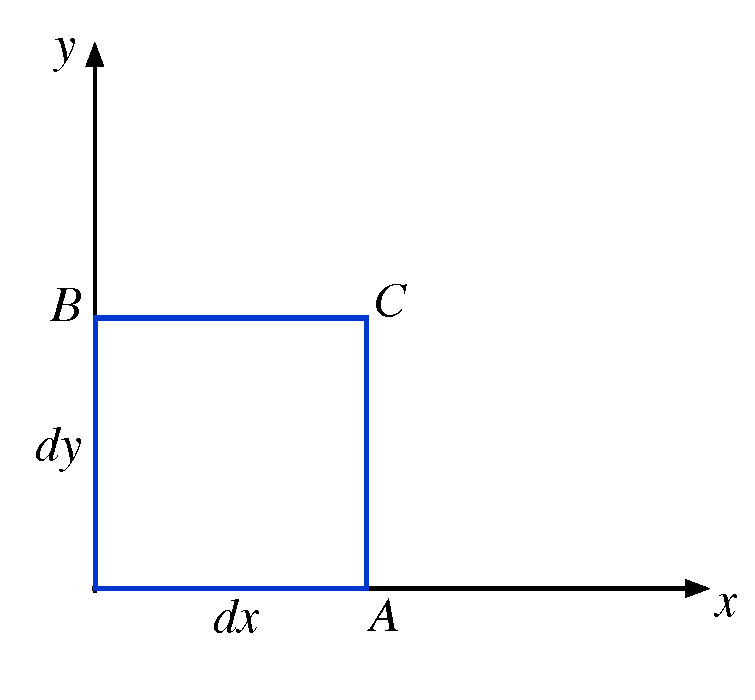
\includegraphics[width=2.5 in]{diferencial.pdf}
	\caption{Elemento diferencial de tamaño $dx \times dy$.}
	\label{diferencial}
\end{figure}

\subsection{Rotación de cuerpo rígido}
Estudiando inicialmente la componente anti-simétrica $\omega$ del tensor $J$ aplicando la transformación sobre el elemento diferencial se tiene respectivamente para los desplazamientos relativos de los puntos $A$, $B$ y $C$:
\begin{align*}
&\begin{Bmatrix}[1.5]
\dd{u}\\
\dd{v}
\end{Bmatrix}_A = \begin{bmatrix}[1.5]
0 &\frac{1}{2}\left(\pdv{u}{y} - \pdv{v}{x}\right)\\
-\frac{1}{2}\left(\pdv{u}{y} - \pdv{v}{x}\right) &0
\end{bmatrix} \begin{Bmatrix}[1.5]
\dd{x}\\
0
\end{Bmatrix} \equiv \begin{Bmatrix}[1.5]
0\\
-\frac{1}{2}\left(\pdv{u}{y} - \pdv{v}{x}\right)\dd{x}
\end{Bmatrix}\\
&\begin{Bmatrix}[1.5]
\dd{u}\\
\dd{v}
\end{Bmatrix}_B = \begin{Bmatrix}[1.5]
\frac{1}{2}\left(\pdv{u}{y} - \pdv{v}{x}\right)\dd{y}\\
0
\end{Bmatrix}\\
&\begin{Bmatrix}[1.5]
\dd{u}\\
\dd{v}
\end{Bmatrix}_C = \begin{Bmatrix}[1.5]
\frac{1}{2}\left(\pdv{u}{y} - \pdv{v}{x}\right)\dd{y}\\
-\frac{1}{2}\left(\pdv{u}{y} - \pdv{v}{x}\right)\dd{x}\\
\end{Bmatrix}
\end{align*}
dando como resultado la configuración deformada de la \cref{crigido}.

Rigurosamente, el elemento experimenta un pequeño cambio de volumen (área) 
considerado como de segundo orden. Claramente esta componente no involucra 
fuerzas internas o tensiones. De otro lado se debe identificar que la rotación 
del elemento esta dada por:
\[\omega = \frac{1}{2}\left(\pdv{u}{y} - \pdv{v}{x}\right)\, .\]
\begin{figure}[H]
\centering
	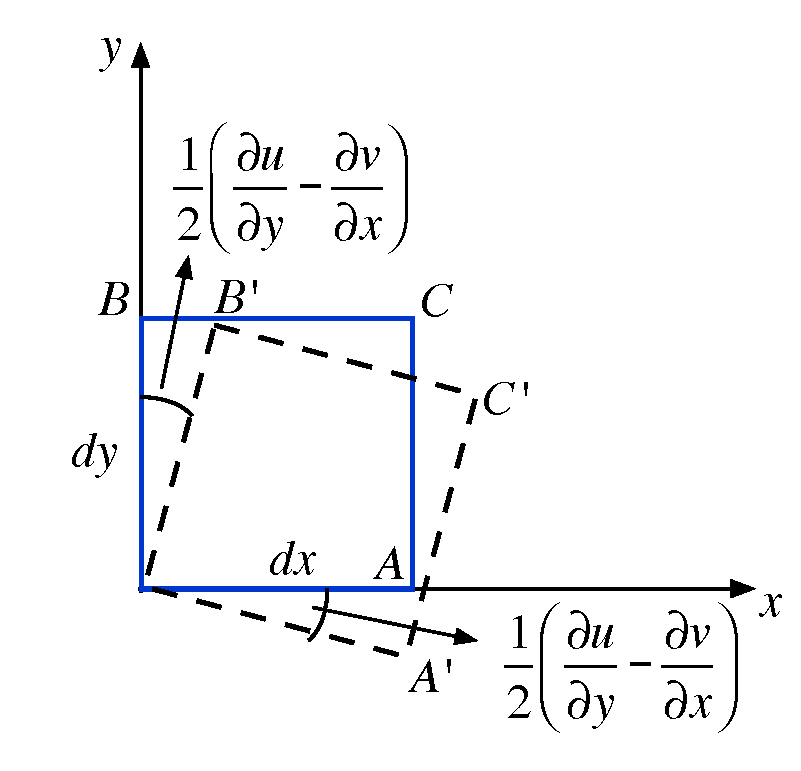
\includegraphics[width=4.0 in]{crigido.pdf}
	\caption{Rotación de cuerpo rígido de un elemento diferencial.}
	\label{crigido}
\end{figure}

\subsection{Componente simétrica $\varepsilon$}
Para el punto A
\[\begin{Bmatrix}[1.5]
\dd{u}\\
\dd{v}
\end{Bmatrix}_A = \begin{bmatrix}[1.5]
\pdv{u}{x} &\frac{1}{2}\left(\pdv{u}{y} + \pdv{v}{x}\right)\\
\frac{1}{2}\left(\pdv{u}{y} + \pdv{v}{x}\right) &\pdv{v}{y}
\end{bmatrix} \begin{Bmatrix}[1.5]
\dd{x}\\
0
\end{Bmatrix} \equiv \begin{Bmatrix}[1.5]
\pdv{u}{x}\dd{x}\\
\frac{1}{2}\left(\pdv{u}{y} + \pdv{v}{x}\right)\dd{y}
\end{Bmatrix}\, .\]

Similarmente, para los puntos $B$ y $C$,
\[\begin{Bmatrix}[1.5]
\dd{u}\\
\dd{v}
\end{Bmatrix}_B = \begin{Bmatrix}[1.5]
\frac{1}{2}\left(\pdv{u}{y} + \pdv{v}{x}\right)\dd{y}\\
\pdv{v}{y}\dd{y}
\end{Bmatrix}\, ,\quad
\begin{Bmatrix}[1.5]
\dd{u}\\
\dd{v}
\end{Bmatrix}_C = \begin{Bmatrix}[1.5]
\pdv{u}{x}\dd{x} + \frac{1}{2}\left(\pdv{u}{y} + \pdv{v}{x}\right)\dd{y}\\
\frac{1}{2}\left(\pdv{u}{y} + \pdv{v}{x}\right)\dd{x} + \pdv{v}{y}\dd{y}
\end{Bmatrix}\, ,\]
resultando en la configuración mostrada en la \cref{strain}.
\begin{figure}[H]
\centering
	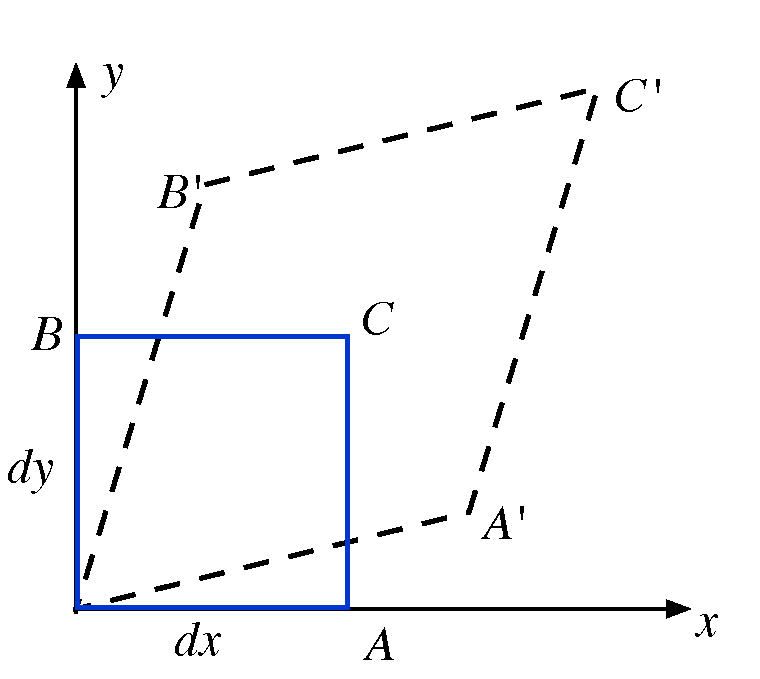
\includegraphics[width=2.5 in]{strain.pdf}
	\caption{Cambio de forma en el elemento diferencial debido a la componente simétrica del gradiente de desplazamientos.}
	\label{strain}
\end{figure}

Ahora, estudiemos de manera individual los efectos de los distintos componentes 
del tensor simétrico $\varepsilon$.

\subsection{Componente escalar, volumétrica o isotrópica}

\begin{align*}
&\begin{Bmatrix}[1.5]
\dd{u}\\
\dd{v}
\end{Bmatrix}_A = \begin{bmatrix}[1.5]
\frac{1}{2}\left( \pdv{u}{x} + \pdv{v}{y}\right) & 0\\
0 & \frac{1}{2}\left(\pdv{u}{x} + \pdv{v}{y}\right)
\end{bmatrix} \begin{Bmatrix}[1.5]
\dd{x}\\
0
\end{Bmatrix} \equiv \begin{Bmatrix}[1.5]
\frac{1}{2}\left(\pdv{u}{x} + \pdv{v}{y}\right)\dd{x}\\
0
\end{Bmatrix}\\
&\begin{Bmatrix}
\dd{u}\\
\dd{v}
\end{Bmatrix}_B = \begin{Bmatrix}[1.5]
0\\
\frac{1}{2}\left(\pdv{u}{x} + \pdv{v}{y}\right) \dd{y}
\end{Bmatrix}\\
&\begin{Bmatrix}[1.5]
\dd{u}\\
\dd{v}
\end{Bmatrix}_C = \begin{Bmatrix}[1.5]
\frac{1}{2}\left(\pdv{u}{x} + \pdv{v}{y}\right)\dd{x}\\
\frac{1}{2}\left(\pdv{u}{x} + \pdv{v}{y}\right)\dd{y}
\end{Bmatrix}
\end{align*}

\begin{figure}[H]
\centering
	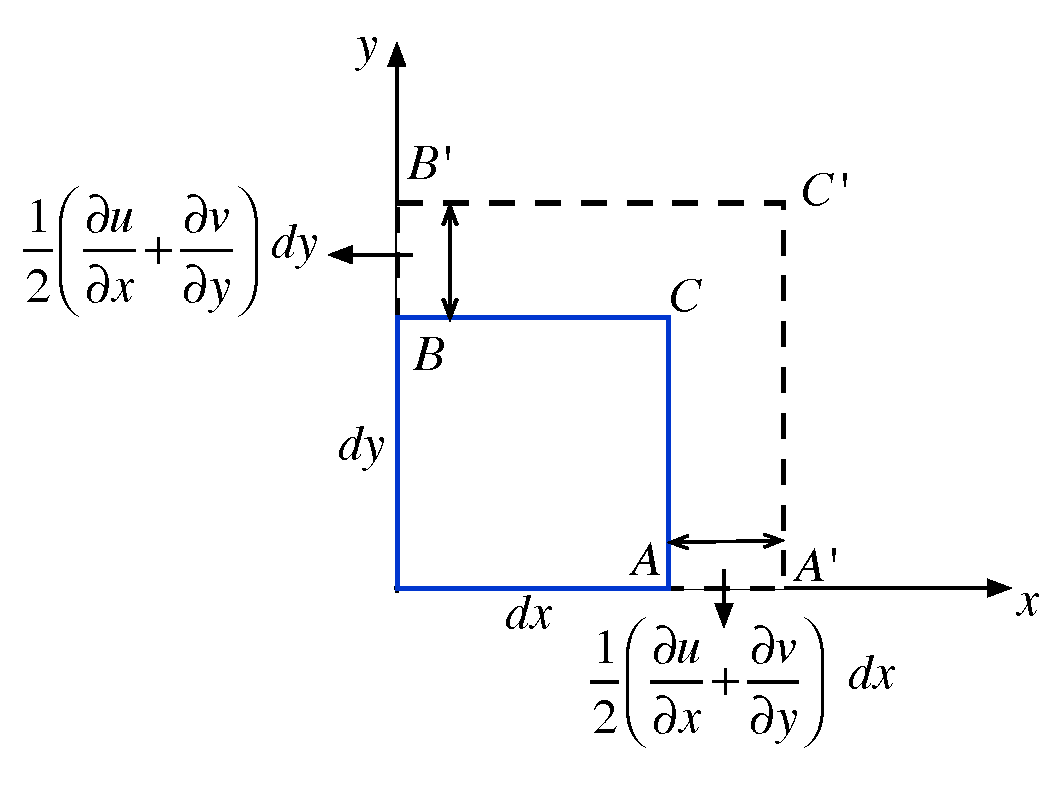
\includegraphics[width=4.0 in]{scalar.pdf}
	\caption{Cambio de forma en el elemento diferencial debido a la componente escalar del gradiente de desplazamientos.}
	\label{scalar}
\end{figure}

\subsection{Componente distorsional}

\begin{align*}
&\begin{Bmatrix}[1.5]
\dd{u}\\
\dd{v}
\end{Bmatrix}_A = \begin{bmatrix}[1.5]
\frac{1}{2}\left(\pdv{u}{x} - \pdv{v}{y}\right) &0\\
0 &-\frac{1}{2}\left(\pdv{u}{x} - \pdv{v}{y}\right)
\end{bmatrix} \begin{Bmatrix}[1.5]
\dd{x}\\
0
\end{Bmatrix} \equiv \begin{Bmatrix}[1.5]
\frac{1}{2}\left(\pdv{u}{x} - \pdv{v}{y}\right)\dd{x}\\
0
\end{Bmatrix}\\
&\begin{Bmatrix}[1.5]
\dd{u}\\
\dd{v}
\end{Bmatrix}_B = \begin{Bmatrix}[1.5]
0\\
-\frac{1}{2}\left(\pdv{u}{x} - \pdv{v}{y}\right) \dd{y}
\end{Bmatrix} \\
&\begin{Bmatrix}[1.5]
\dd{u}\\
\dd{v}
\end{Bmatrix}_C = \begin{Bmatrix}[1.5]
\frac{1}{2}\left(\pdv{u}{x} - \pdv{v}{y}\right) \dd{x}\\
-\frac{1}{2}\left(\pdv{u}{x} - \pdv{v}{y}\right)\dd{y}
\end{Bmatrix}
\end{align*}

\begin{figure}[H]
\centering
	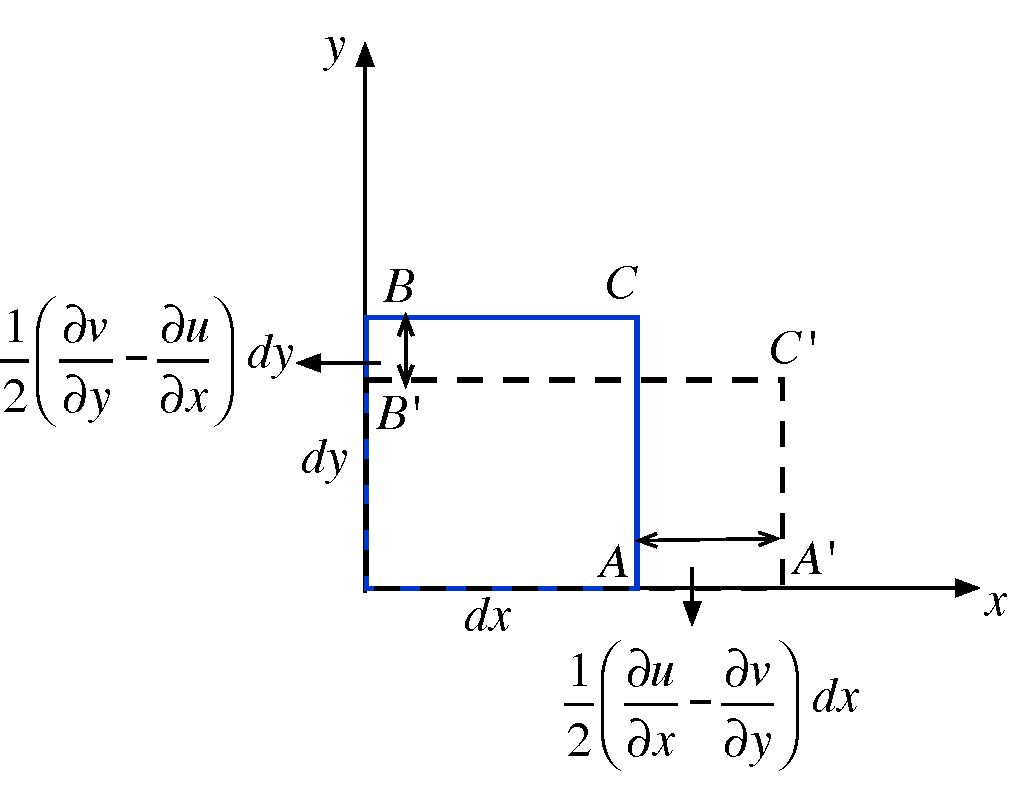
\includegraphics[width=3.0 in]{1dist.pdf}
	\caption{Cambio de forma en el elemento diferencial debido a la primera componente distorsional del tensor de deformaciones unitarias.}
	\label{1dist}
\end{figure}

\begin{align*}
&\begin{Bmatrix}[1.5]
\dd{u}\\
\dd{v}
\end{Bmatrix}_A = \begin{bmatrix}[1.5]
0 &\frac{1}{2}\left(\pdv{u}{y} + \pdv{v}{x}\right)\\
\frac{1}{2}\left(\pdv{u}{y} + \pdv{v}{x}\right) &0
\end{bmatrix} \begin{Bmatrix}[1.5]
\dd{x}\\
0
\end{Bmatrix} \equiv \begin{Bmatrix}[1.5]
0\\
\frac{1}{2}\left(\pdv{u}{y} + \pdv{v}{x}\right) \dd{x}
\end{Bmatrix}\\
&\begin{Bmatrix}[1.5]
\dd{u}\\
\dd{v}
\end{Bmatrix}_B = \begin{Bmatrix}[1.5]
\frac{1}{2}\left(\pdv{u}{y} + \pdv{v}{x}\right) \dd{y}\\
0
\end{Bmatrix}\\
&\begin{Bmatrix}[1.5]
\dd{u}\\
\dd{v}
\end{Bmatrix}_C = \begin{Bmatrix}[1.5]
\frac{1}{2}\left(\pdv{u}{y} + \pdv{v}{x}\right) \dd{y}\\
\frac{1}{2}\left(\pdv{u}{y} + \pdv{v}{x}\right) \dd{x}
\end{Bmatrix}
\end{align*}

\begin{figure}[H]
\centering
	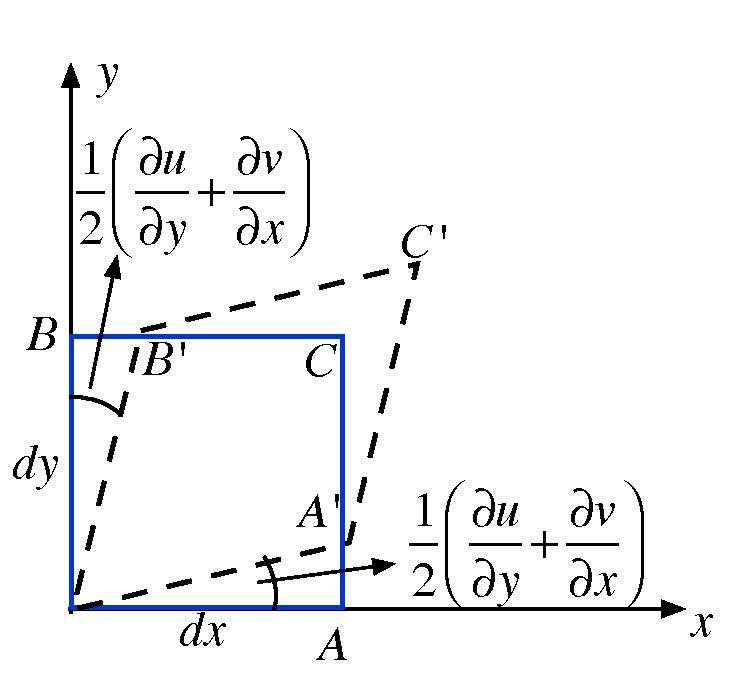
\includegraphics[width=3.0 in]{2dist.pdf}
	\caption{Cambio de forma en el elemento diferencial debido a la segunda componente distorsional del tensor de deformaciones unitarias.}
	\label{2dist}
\end{figure}

Ahora, en el argot ingenieril es común a cada término de la componente 
simétrica del tensor gradiente de desplazamientos asignarle una nomenclatura 
particular. Para generalizar la definición consideremos el tensor $\varepsilon$ 
expresado en coordenadas cartesianas.
\[	
[\varepsilon] =
\begin{bmatrix}[2]
  \pdv{u}{x} & \frac{1}{2} \left(\pdv{u}{y} + \pdv{v}{x}\right)
  & \frac{1}{2} \left(\pdv{u}{z} + \pdv{w}{x}\right) \\
  \frac{1}{2} \left(\pdv{v}{x} + \pdv{u}{y}\right)  & \pdv{v}{y}
  & \frac{1}{2}	\left(\pdv{v}{z} + \pdv{w}{y}\right) \\
  \frac{1}{2} \left(\pdv{w}{x} + \pdv{u}{z}\right) & \frac{1}{2} 
  \left(\pdv{w}{y} + \pdv{v}{z}\right)  & \pdv{w}{z}
\end{bmatrix}\, ,\]
o, escrito de otra forma: 
\[	
[\varepsilon] =
\begin{bmatrix}[2]
  \varepsilon_{xx} & \dfrac{1}{2} \gamma_{xy} & \dfrac{1}{2} \gamma_{xz}  \\
  \dfrac{1}{2} \gamma_{xy}  & \varepsilon_{yy} & \dfrac{1}{2}  \gamma_{yz}  \\
  \dfrac{1}{2} \gamma_{xz} & \dfrac{1}{2} \gamma_{yz}  &  \varepsilon_{zz}
\end{bmatrix}\]\\

En donde $\varepsilon_{xx}$, $\varepsilon_{yy}$ y $\varepsilon_{zz}$ son conocidas como deformaciones axiales o normales y  $\gamma_{xy}$ ,$ \gamma_{xz}$  y $\gamma_{yz}$  como deformaciones angulares o deformaciones por cortante. 

Por otro lado, la componente rotacional podría escribirse
\[	
[\omega] =
\begin{bmatrix}
  0 & \omega_{xy}  &  \omega_{xz} \\
  -\omega_{xy}  & 0 &  \omega_{yz} \\
  -\omega_{xz}  & -\omega_{yz}  &  0
\end{bmatrix}\, ,\]
en donde $\omega_{xy}$, $\omega_{xz}$ y  $\omega_{yz}$ representan la rotación 
de cuerpo rígido respecto a los ejes $z$, $y$ y $x$ respectivamente.

Para terminar, el tensor $\varepsilon$ en coordenadas cilíndricas está definido 
como: 
\[	
[\varepsilon] =
\begin{bmatrix}[2]
  \varepsilon_{rr} & \dfrac{1}{2} \gamma_{r\theta} & \dfrac{1}{2} \gamma_{rz}  
  \\
  \dfrac{1}{2} \gamma_{r\theta}  & \varepsilon_{\theta\theta} & 
  \dfrac{1}{2}  \gamma_{\theta z}  \\
  \dfrac{1}{2} \gamma_{rz} & \dfrac{1}{2} \gamma_{\theta z}  &  
  \varepsilon_{zz}
\end{bmatrix}\, ,\]
en donde
\begin{align*}	
    &\varepsilon_{rr} = \pdv{u}{r}\, ,\qquad
    \varepsilon_{\theta \theta} = \frac{u}{r} + \frac{1}{r}\pdv{v}{\theta}\, ,
    \quad \varepsilon_{zz} = \pdv{w}{z}\, ,\\
    &\gamma_{r \theta} = \frac{1}{r} \pdv{u}{\theta} + \pdv{v}{r} - 
    \frac{v}{r}\, ,\quad
    \gamma_{\theta z} = \pdv{v}{z} + \frac{1}{r}\pdv{w}{\theta}\, ,\quad
    \gamma_{rz}	 = \pdv{u}{z} + \pdv{w}{r}\, .
\end{align*}

\section*{Ejemplo}

El campo de desplazamientos para la cuña auto-soportada mostrada en la \cref{wedge} esta dado por:
\begin{equation*}	
	u = \frac{S}{E} K_1 (\nu ,\phi) (x - \ell \cos\phi)\qquad
	v =  - \frac{S}{E} K_2 (\nu ,\phi) y
\end{equation*}
donde $u$ y $v$ corresponden a los desplazamientos en las direcciones horizontal y vertical respectivamente y ${K_1}\left( {\nu ,\phi } \right)$ y ${K_2}\left( {\nu ,\phi } \right)$ son constantes que dependen del semi-ángulo de la cuña y del material. $E$ es una constante que depende del material. 
\begin{figure}[H]
\centering
	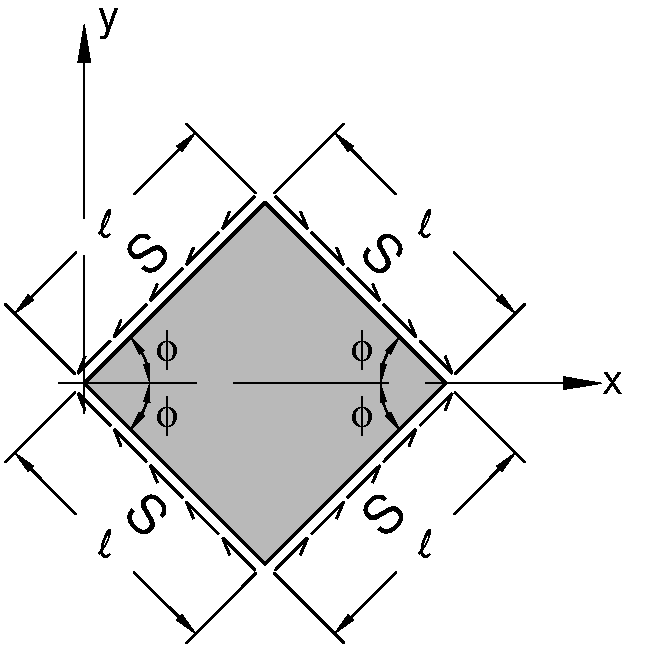
\includegraphics[width=2.8 in]{wedge.pdf}
	\caption{Cuña auto-soportada.}
	\label{wedge}
\end{figure}

\begin{itemize}
\item[•] Esbozar la configuración deformada (final) de la cuña
\item[•] Los tensores gradiente de desplazamientos $J$, deformaciones unitarias $\epsilon$ y rotaciones $\omega$.
\item[•] Determinar las direcciones de máximo cambio de tamaño y máxima rotación.
\end{itemize}

Para esbozar la configuración deformada de la cuña es preciso evaluar el campo 
de desplazamientos en puntos de la misma. Debido a la linealidad de las 
funciones del campo de desplazamientos $u$ y $v$ y por la simetría del 
problema miramos lo que pasa en cada una de las esquinas
\footnote{Para funciones de desplazamiento más complejas puede ser preciso usar 
métodos más elaborados para la evaluación de dichas funciones.}. Es decir, 
evaluamos los desplazamientos en los puntos $A = (0,0)$,  $B = (\ell \cos\phi, 
\ell \sin\phi)$, $C = (\ell \cos\phi, -\ell \sin\phi)$ y $D = (2\ell 
\cos\phi,0)$. En la \cref{wedgedef} se muestra esquemáticamente en linea 
punteada la configuración deformada de la cuña. Nótese  como los puntos 
ubicados en el eje de simetría $A-D$ solo tienen desplazamiento en $x$, $u$, 
mientras que los puntos en el eje de simetría $B-C$ solo en $y$, $v$. El punto 
central del medio continuo no se desplaza. 
\begin{figure}[H]
\centering
	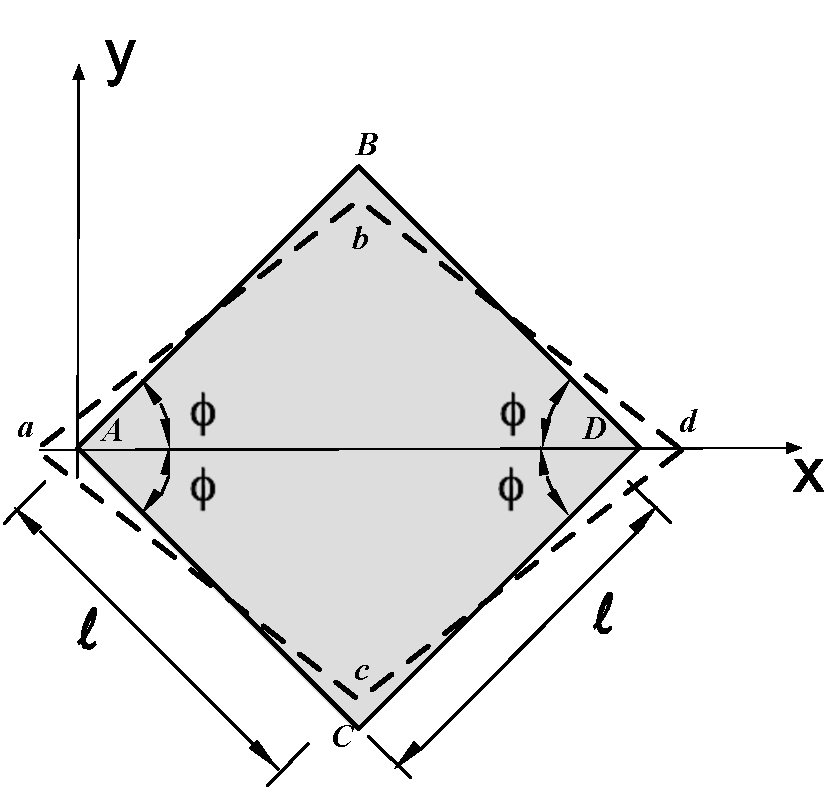
\includegraphics[width=3.0 in]{wedgedef.pdf}
	\caption{Configuración final Cuña auto-soportada.}
	\label{wedgedef}
\end{figure}

Por otro lado, el tensor gradiente de desplazamientos está dado por: 
\[J = \frac{S}{E}\begin{bmatrix}[1.5]
K_1(\nu, \phi) &0\\
0 &-K_2(\nu, \phi)
\end{bmatrix}\]
y, en este caso, se tiene que \(\varepsilon  \equiv J\).

Luego, las rotaciones de cuerpo rígido son nulas
\[\omega  = 0\, .\]

Nótese que el tensor $\varepsilon$ ya está escrito en sus valores principales, 
lo que quiere decir que las deformaciones axiales máximas están dadas por: 
$\frac{S}{E} K_1(\nu, \phi)$ como el estiramiento máximo, y $\frac{S}{E} 
K_2(\nu, \phi)$ como el acortamiento máximo.

\subsection{Ejemplo: Barra sometida a su peso propio}

En la  \cref{BarApo} se muestra una barra de sección circular de radio $R$, 
altura $H$, fija en su extremo inferior y que está sometida solamente a la 
acción de su propio peso. Se indica el campo de desplazamientos en el sistema 
coordenado $xyz$.
\begin{equation*}	
	u = \nu \dfrac{\gamma}{E} z x\, ,
	\hspace{1cm}
	v = \nu \dfrac{\gamma}{E} z y\, ,
	\hspace{1cm}
	w = -\dfrac{\gamma}{2E} z^2 - \dfrac{\gamma \nu}{2E} 
	(x^2+y^2)+\dfrac{\gamma}{2E} H^2\, , 
\end{equation*}
donde $u,v,w$ son los desplazamientos asociados a los ejes $x,y,z$,  
respectivamente. $E$, $\gamma$ y $\nu$ son constantes del material.	
\begin{figure}[h]
	\centering
	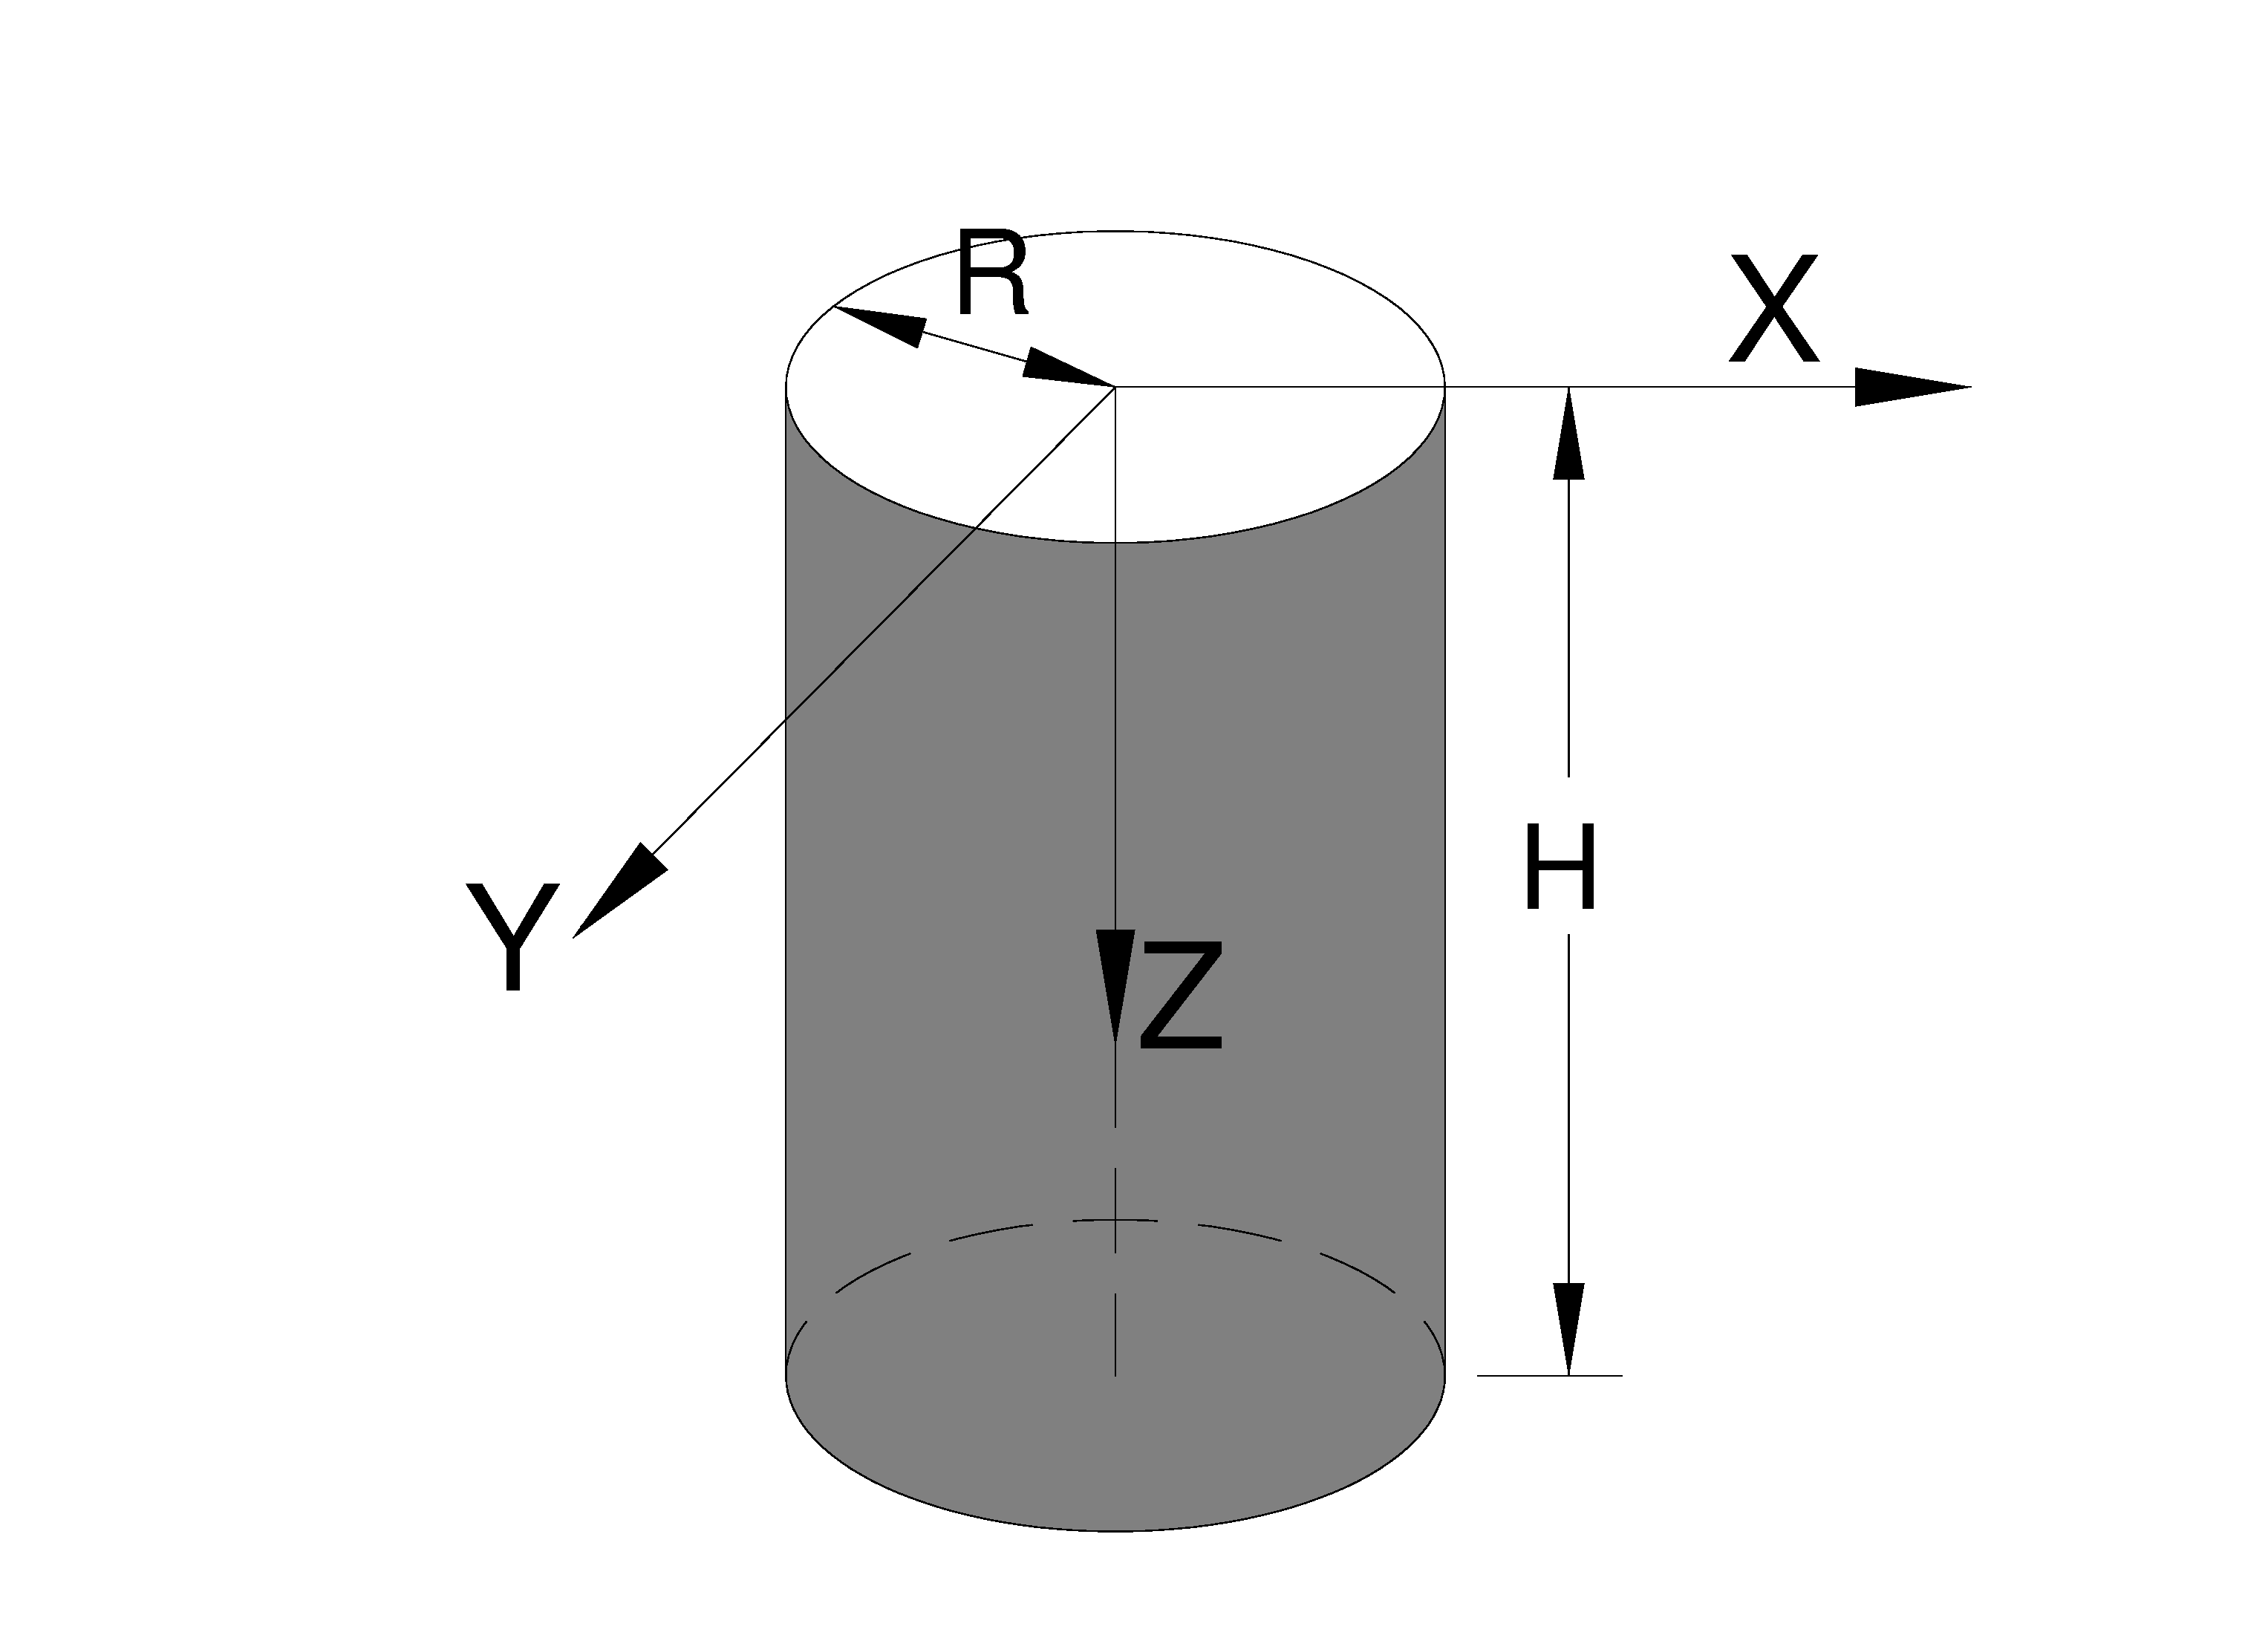
\includegraphics[height=6cm]{barraapoyada.pdf}
	\caption{Barra apoyada}
	 \label{BarApo}
\end{figure}\\

\begin{enumerate}

\item[•] Esboce la configuración deformada de la barra.
	
\subsubsection{Solución:}
	
Para esbozar una configuración deformada lo hacemos a partir del campo de 
desplazamientos $u$, $v$, $w$. Para realizarla  hagamos un corte transversal 
(plano $xy$) y un corte longitudinal (plano $xz$) y evaluemos que pasa con los 
desplazamientos en algunos puntos de la frontera.
\begin{align*}
&x = 0,  \;\;  y = 0,  \;\; z = 0.  \;\;   \Longrightarrow  \;\; u = 0,  
\;\;\;   v = 0, \;\;\;   w = \dfrac{\gamma}{2E} H \\
&x =\pm R,  \;\;  y = 0,  \;\; z = 0.  \;\;   \Longrightarrow  \;\; u = 0,  
\;\;\;   v = 0, \;\;\;   w = - \dfrac{\gamma \nu}{2E} R^2 +  \dfrac{\gamma}{2E} 
H^2\\
&x =0,  \;\;  y = \pm R,  \;\; z = 0.  \;\;   \Longrightarrow  \;\; u = 0,  
\;\;\;   v = 0, \;\;\;   w = - \dfrac{\gamma \nu}{2E} R^2 +  \dfrac{\gamma}{2E} 
H^2\\
&x = 0,  \;\;  y = 0,  \;\; z = H.  \;\;   \Longrightarrow  \;\; u = 0,  
\;\;\;   v = 0, \;\;\;   w = 0  \\
&x = \pm R,  \;\;  y = 0,  \;\; z = H.  \;\;   \Longrightarrow  \;\; u =\pm \nu 
\dfrac{\gamma}{E} H R,   \;\;\;   v = 0, \;\;\;   w = - \dfrac{\gamma \nu}{2E} 
R^2\\
&x = 0,  \;\;  y = \pm R,  \;\; z = H.  \;\;   \Longrightarrow  \;\; u =0,   
\;\;\;   v = \pm \nu \dfrac{\gamma}{E} H R, \;\;\;   w = - \dfrac{\gamma 
\nu}{2E} R^2
\end{align*}

En la figura \cref{ConDef} aparecen la configuración inicial (línea punteada) y 
final del elemento. 
\begin{figure}[h]
	\centering
	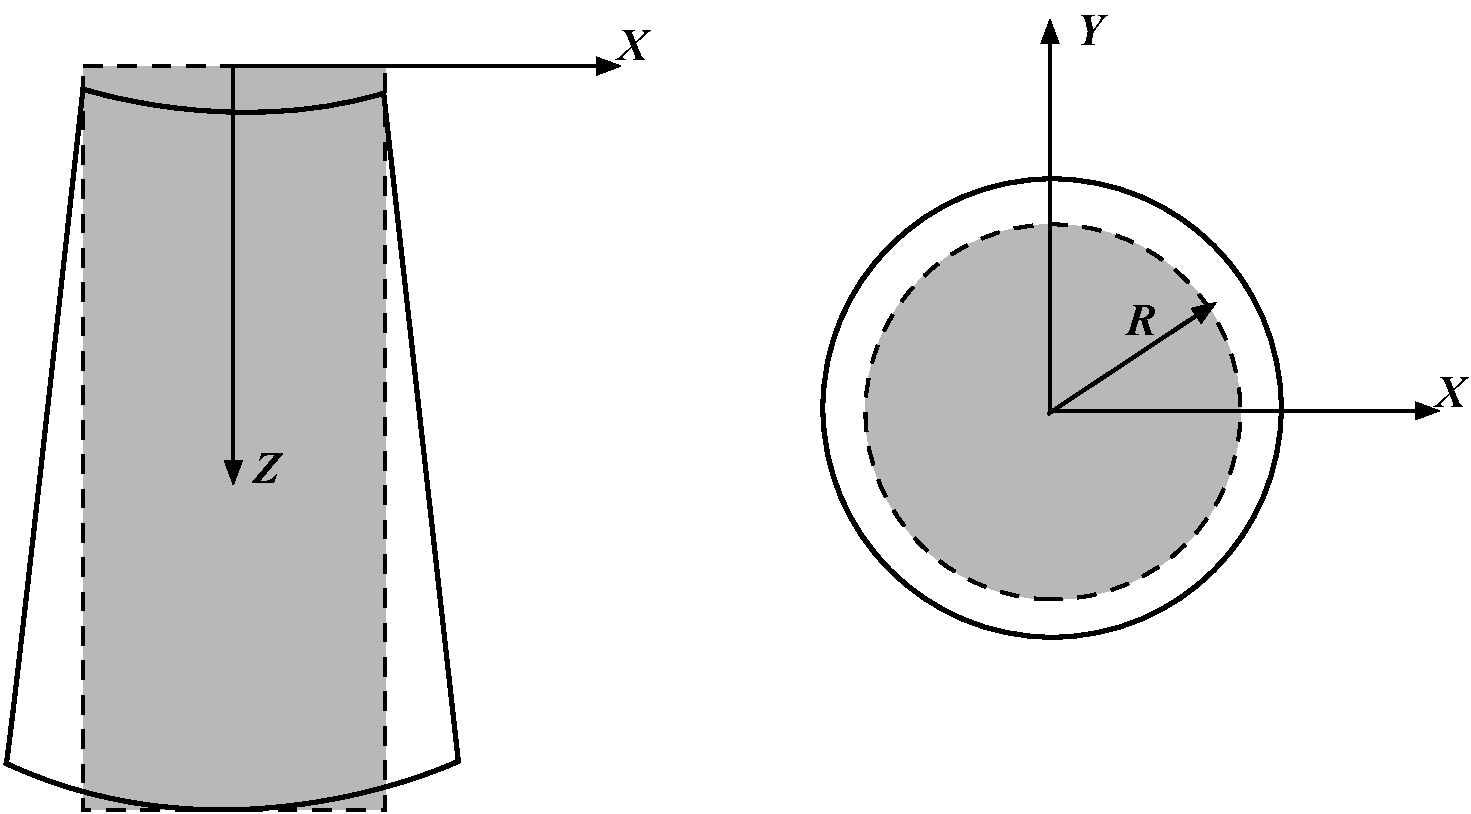
\includegraphics[height=4.5cm]{Configura.pdf}
	\caption{Cortes con configuración final}
	 \label{ConDef}
\end{figure}
%	
\item[•] Calcule el tensor gradiente de desplazamientos y descompóngalo en 
$[\varepsilon]$ (simétrico) y $[\omega]$ (asimétrico).
	
\subsubsection{Solución:}

El tensor gradiente de desplazamientos está dado por: 
\[[D]	=   \dfrac{\gamma}{E}
\begin{bmatrix}
 \nu  z & 0 &  \nu  x\\
 0 &  \nu  z &  \nu  y\\
 - \nu x & - \nu  y &  - z
\end{bmatrix}\, . \]
	
El tensor  $\varepsilon$ y $\omega$ están dados por: 
\[[\varepsilon] = \dfrac{\gamma}{E}
\begin{bmatrix}
  \nu  z & 0 &  0\\
  0 &  \nu  z &  0\\
  0 & 0 &  -  z
\end{bmatrix}\, ,
\hspace{2cm}
[\omega]
= \dfrac{\gamma}{E}
\begin{bmatrix}
  0 & 0 &  \nu x\\
  0 & 0 &  \nu y\\
 -\nu x & -\nu  y &  0
\end{bmatrix}\, . \]

\item[•] ¿Cuáles son los valores máximos y mínimos de las deformaciones 
axiales y en que puntos se presentan? 
	
\subsubsection{Solución:}
\begin{align*}	
&\varepsilon_{xx} =  \nu \dfrac{\gamma}{E} z  \;\; \Longrightarrow  \;\; 
\varepsilon_{\min} = 0  \;\;\; (z=0),  \;\;\;\;  \varepsilon_{\max} = \nu 
\dfrac{\gamma}{E} H \;\;\; (z=H) \\
&\varepsilon_{yy} =  \nu \dfrac{\gamma}{E} z  \;\; \Longrightarrow  \;\; 
\varepsilon_{\min} = 0  \;\;\; (z=0),  \;\;\;\;  \varepsilon_{\max} = \nu 
\dfrac{\gamma}{E} H \;\;\; (z=H)\\
&\varepsilon_{zz} =  - \dfrac{\gamma}{E} z  \;\; \Longrightarrow  \;\; 
\varepsilon_{\min} = 0  \;\;\; (z=0),  \;\;\;\;  \varepsilon_{\max} = - 
\dfrac{\gamma}{E} H \;\;\; (z=H)
\end{align*}

\item[•] ¿Cuáles son los valores máximos y mínimos de los desplazamientos 
$u$, $v$ y $w$ y en que puntos se presentan?

\subsubsection{Solución:}
\begin{align*}
&u =  \nu \dfrac{\gamma}{E} zx  \;\; \Longrightarrow  \;\; u_{\min} = 0  \;\;\; 
(x=0),  \;\;\;\;  u_{\max} =\abs{ \nu \dfrac{\gamma}{E} HR} \;\;\; (z=H, 
x=\abs{R}) \\
&v =  \nu \dfrac{\gamma}{E} zy  \;\; \Longrightarrow  \;\; v_{\min} = 0  \;\;\; 
(y=0),  \;\;\;\;  v_{\max} =\abs{ \nu \dfrac{\gamma}{E} HR} \;\;\; (z=H, 
y=\abs{R})
\end{align*}

Para el caso del desplazamiento en $z$ los máximos dependen de la relación 
entre $H^2$ y $R^2=x^2 + y^2$. Supongamos $H>R$. 
	

\[w_{\min} = 0  \;\;\; ( x=y=0,z=H),  \;\;\;\;  w_{\max} = \dfrac{\gamma}{2E} 
H^2  \;\;\; (x=y=z=0)\]

\item[•]¿Existen puntos exentos de rotación de cuerpo rígido?, responda 
sí o no y justifique su respuesta.

\subsubsection{Solución:}

Sí, si existen puntos exentos de rotación. La línea longitudinal cuando $x=y=0$ 
no experimenta rotación de cuerpo rígido. 

\item[•]¿Es posible encontrar puntos sometidos a deformación angular?, responda 
sí o no y justifique su respuesta.

\subsubsection{Solución:}

Sí es posible. Como puede verse en el tensor  $\varepsilon$ los valores 
principales son diferentes, por lo es posible encontrar alguna dirección 
sometida a deformación angular.

\end{enumerate}

\subsubsection{Tarea}

Describa la configuración deformada de las partículas. 

\section{Ejercicios propuestos}

\begin{enumerate}

\item \label{ejer:trans_lineal} En la  figura \ref{fig:elipse} se muestra la 
configuración inicial y final en donde las coordenadas puntos son A, B, C y D 
son $A=(1,1)$, $B=(-1,-1)$, $C=(-\sqrt{2}/2,\sqrt{2}/2)$, 
$D=(\sqrt{2}/2,-\sqrt{2}/2)$. Sabiendo que $\vec{r}$ es el vector de posici\'on 
original, $\vec{\rho}$ es el vector de posición final y  $\vec{\vartriangle}$ 
es vector de desplazamiento 

\begin{enumerate}
\item Determinar la matriz de desplazamientos lineales $[D]$ tal que	
$\vec{\vartriangle}=  D  \vec{r}$. 
\item Determinar la matriz de transformación lineal $[A]$ tal que 
$\vec{\rho}= A  \vec{r}$	
\item Descomponer $[D]$ en componente simétrica y componente asimétrica. 
Mostrar gráficamente lo efectos. 	
\item  Usando el circulo de Mohr, determinar las direcciones principales y los 
valores propios de la matriz de transformación lineal simétrica.
\end{enumerate}

\begin{figure}[H]
    \centering	
    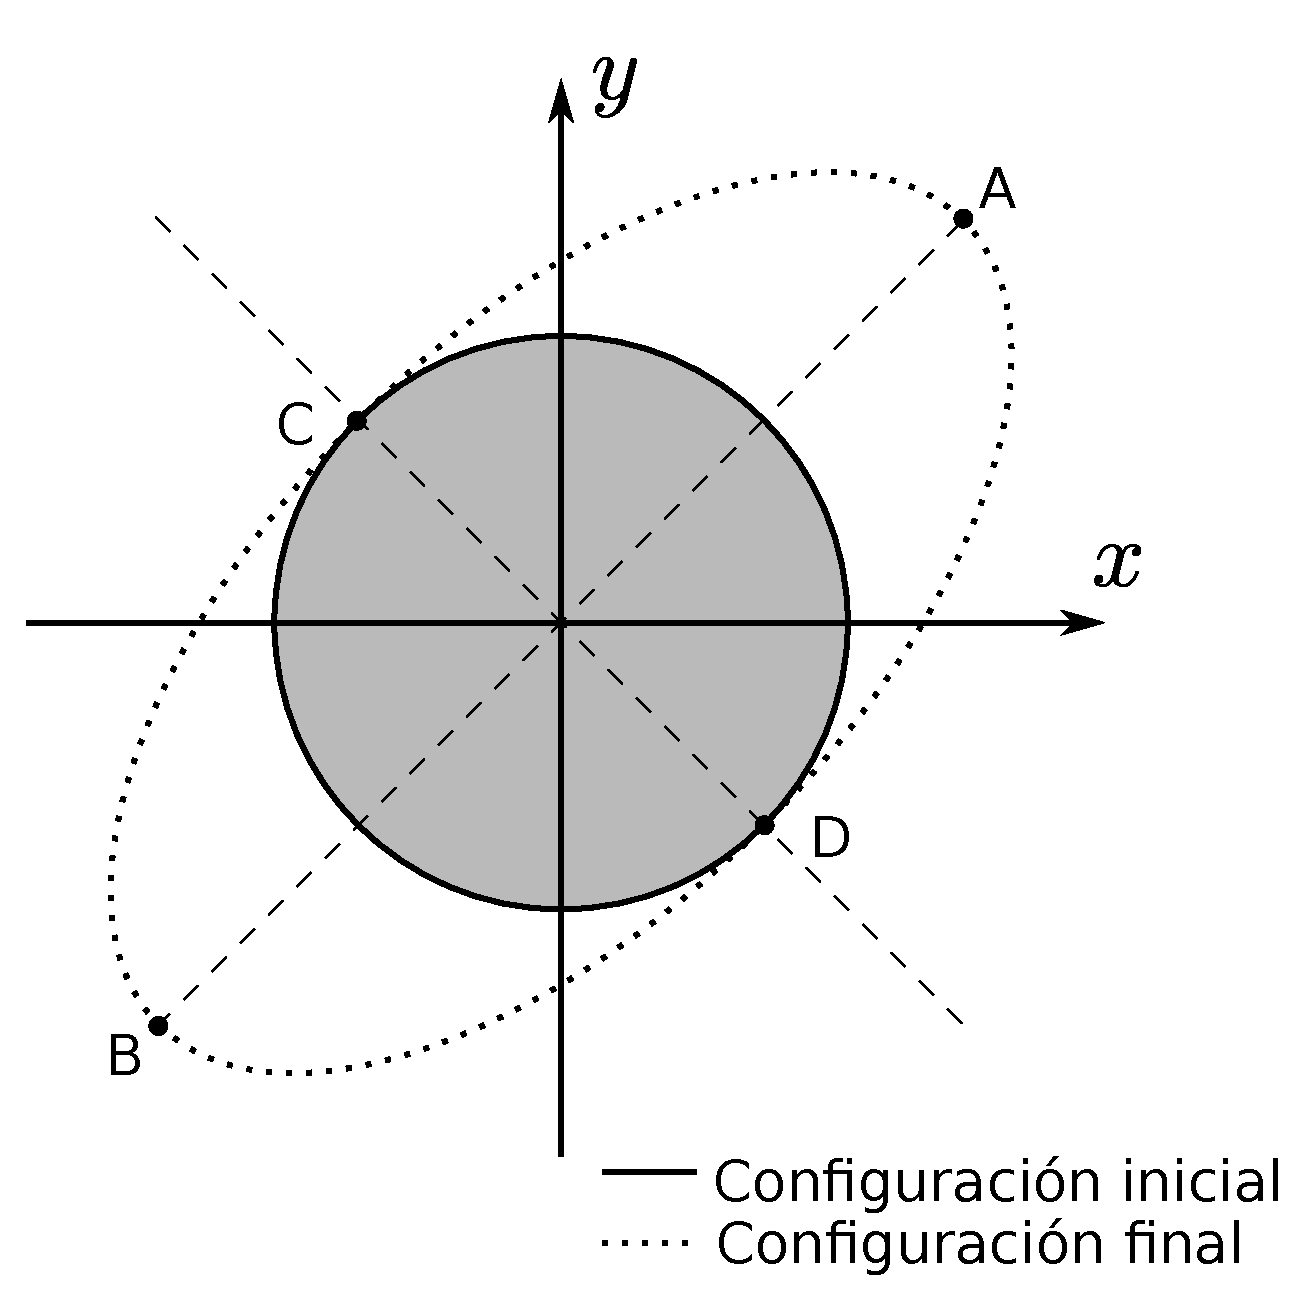
\includegraphics[scale=0.4]{Elipse.pdf}
    \caption{Representación gráfica de una transformación lineal.}
    \label{fig:elipse}
\end{figure}
	
\item  \label{punto02_d} En la figura \cref{Triangulo} se muestra la 
configuración inicial y final (linea punteada) del un triángulo de lado 
unitario formado por los puntos A, B, C. Para pasar de la configuración inicial 
a la final se aplica una trasformación lineal de desplazamientos $[D]$, tal que 
$\lbrace{\Delta}\rbrace = [D]\cdot\lbrace{r}\rbrace$, donde $\Delta$ es el 
vector desplazamiento, y $r$ es el vector posici\'on inicial.

\begin{figure}[H]
	\centering
	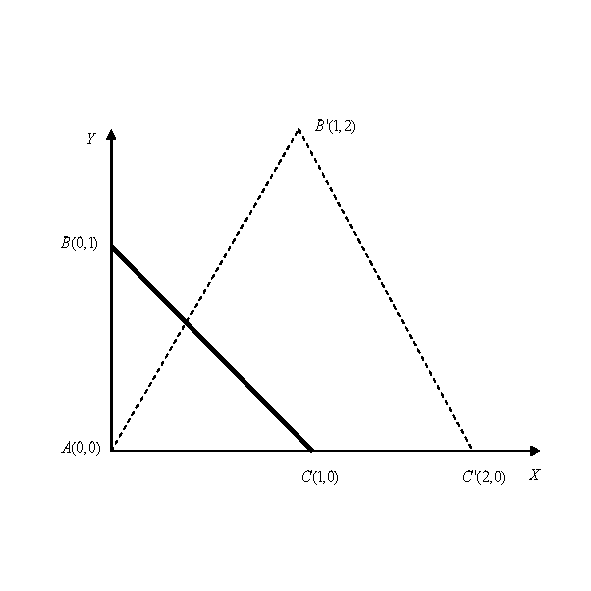
\includegraphics[height=9cm]{Triangulo.pdf} 
	\caption{Configuraciones inicial y deformada}
	\label{Triangulo}
\end{figure}

\begin{enumerate}
\item Determinar la transformación lineal $[D]$, y descomponerla en sus componente simétrica $[\varepsilon]$ y asimétrica $[\omega]$.
\item Determinar las direcciones principales de la transformación $[D]$. Es 
posible usar el círculo de Mohr.
\item Mostrar matemática y gráficamente el efecto independiente de las diferentes componentes del tensor lineal de desplazamientos. Las componentes a considerar son la isotrópica, las distorsionales y la rotación de cuerpo rígido, tal que $[D] = p[I] + [S] +[C] + [\omega]$
\item Escribir en sus direcciones principales la componente simétrica $[\varepsilon]$ de la transformación $[D]$.
\end{enumerate}


\item  \label{punto03_d} La figura \cref{Rectangulo} muestra un rectángulo 
infinitesimal de lado $b$ y altura $h$ en la configuración sin deformar el 
cual es deformado por alguna acci\'on externa y dicha deformación se describe 
como la superposición lineal de varias deformaciones individuales, las cuales 
se dan a continuación: 
\begin{enumerate}
\item $ {\varepsilon_1}=\left(\begin{array}{ccc}
d & 0 \\ 
0 & d 
\end{array}\right) \enspace $

\item $ {\varepsilon_2}=\left(\begin{array}{ccc}
e & 0 \\ 
0 & -e 
\end{array}\right) \enspace $

\item ${\varepsilon_3}=\left(\begin{array}{ccc}
0 & f \\ 
f & 0 
\end{array}\right) \enspace $
\end{enumerate}
	
\begin{figure}[H]		
	\centering	
	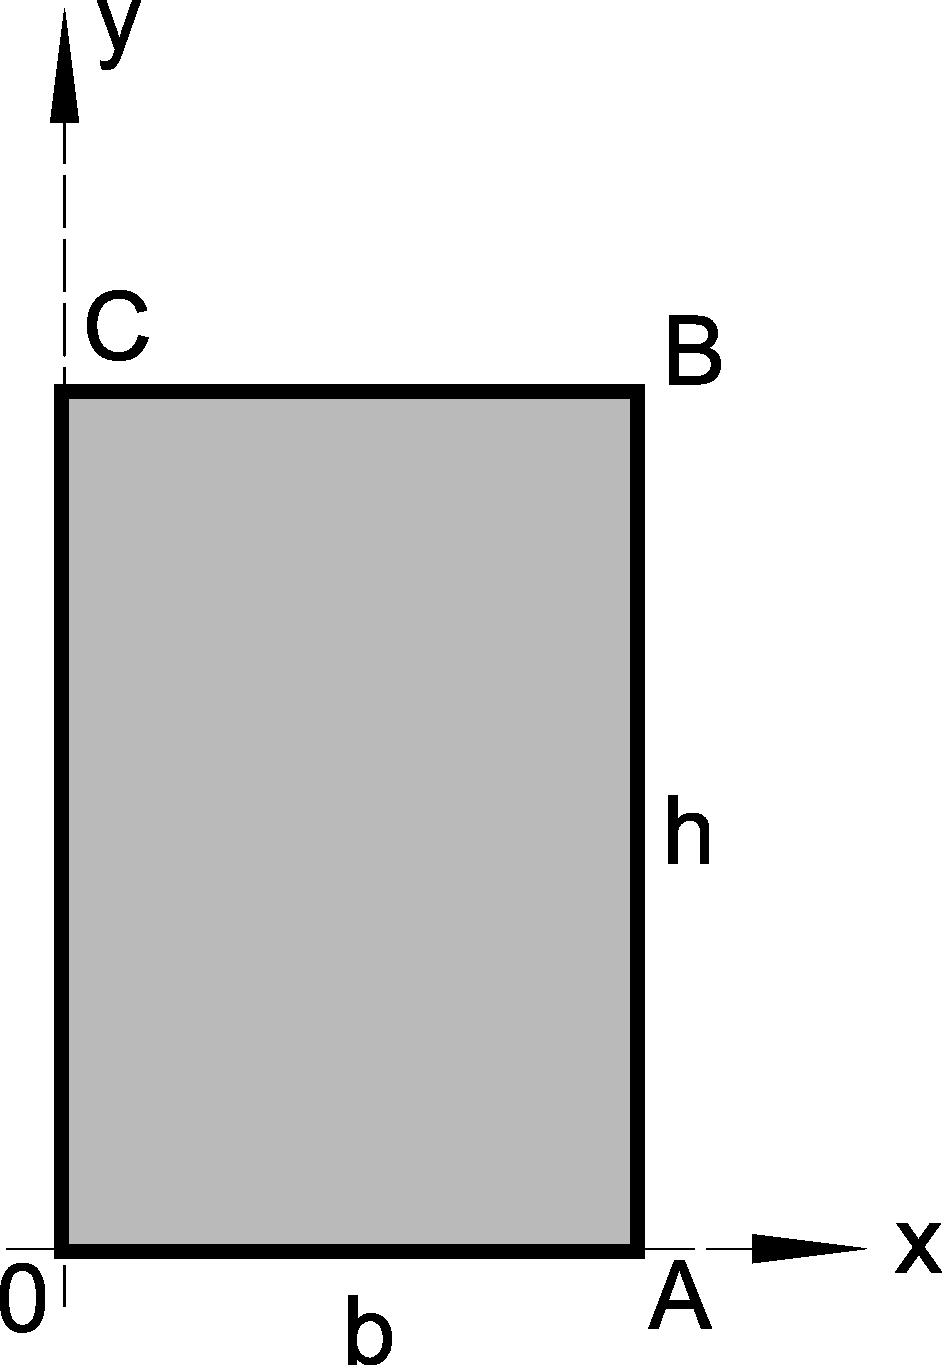
\includegraphics[scale=0.25]{Rectangulo.pdf}
	\caption{Rectángulo en la configuración no deformada.}
	\label{Rectangulo}
\end{figure}

Se pide determinar lo siguiente:
	
\begin{enumerate}
	\item Calcular los desplazamientos de los puntos $A$, $B$ y $C$ para cada 
	uno de los estados de deformación y dibujar las configuraciones deformadas.
	\item Si se sabe que las dimensiones del rectángulo $b=1.00$ y $h=1.00$ y 
	los valores de las transformaciones son $d=0.01$, $e=0.005$ y $f=0.0025$. 
	Calcular las direcciones principales y los valores propios para la 
	superposición lineal de las deformaciones. 	
\end{enumerate}

\item  \label{punto04_d} En la figura \cref{BarraColgada} se muestra una barra 
de sección circular de radio $R$, altura H, soportada de su extremo superior y 
que está sometido solamente a la acción de su peso propio. El campo de 
desplazamientos $u,v,w$ en el sistema coordenado $xyz$ de para la barra está 
dado por:
\[u = -\nu \dfrac{\gamma}{E} z x\, ,  \hspace{1cm}	
v = -\nu \dfrac{\gamma}{E} z y\, ,  \hspace{1cm}	
w = \dfrac{\gamma}{2E} z^2 +\dfrac{\gamma \nu}{2E} (x^2+y^2)-\dfrac{\gamma}{2E} 
H^2\ ,\]
donde $E$, $\gamma$ y $\nu$ son constantes del material (positivas). 
	
\begin{figure}[H]
	\centering
	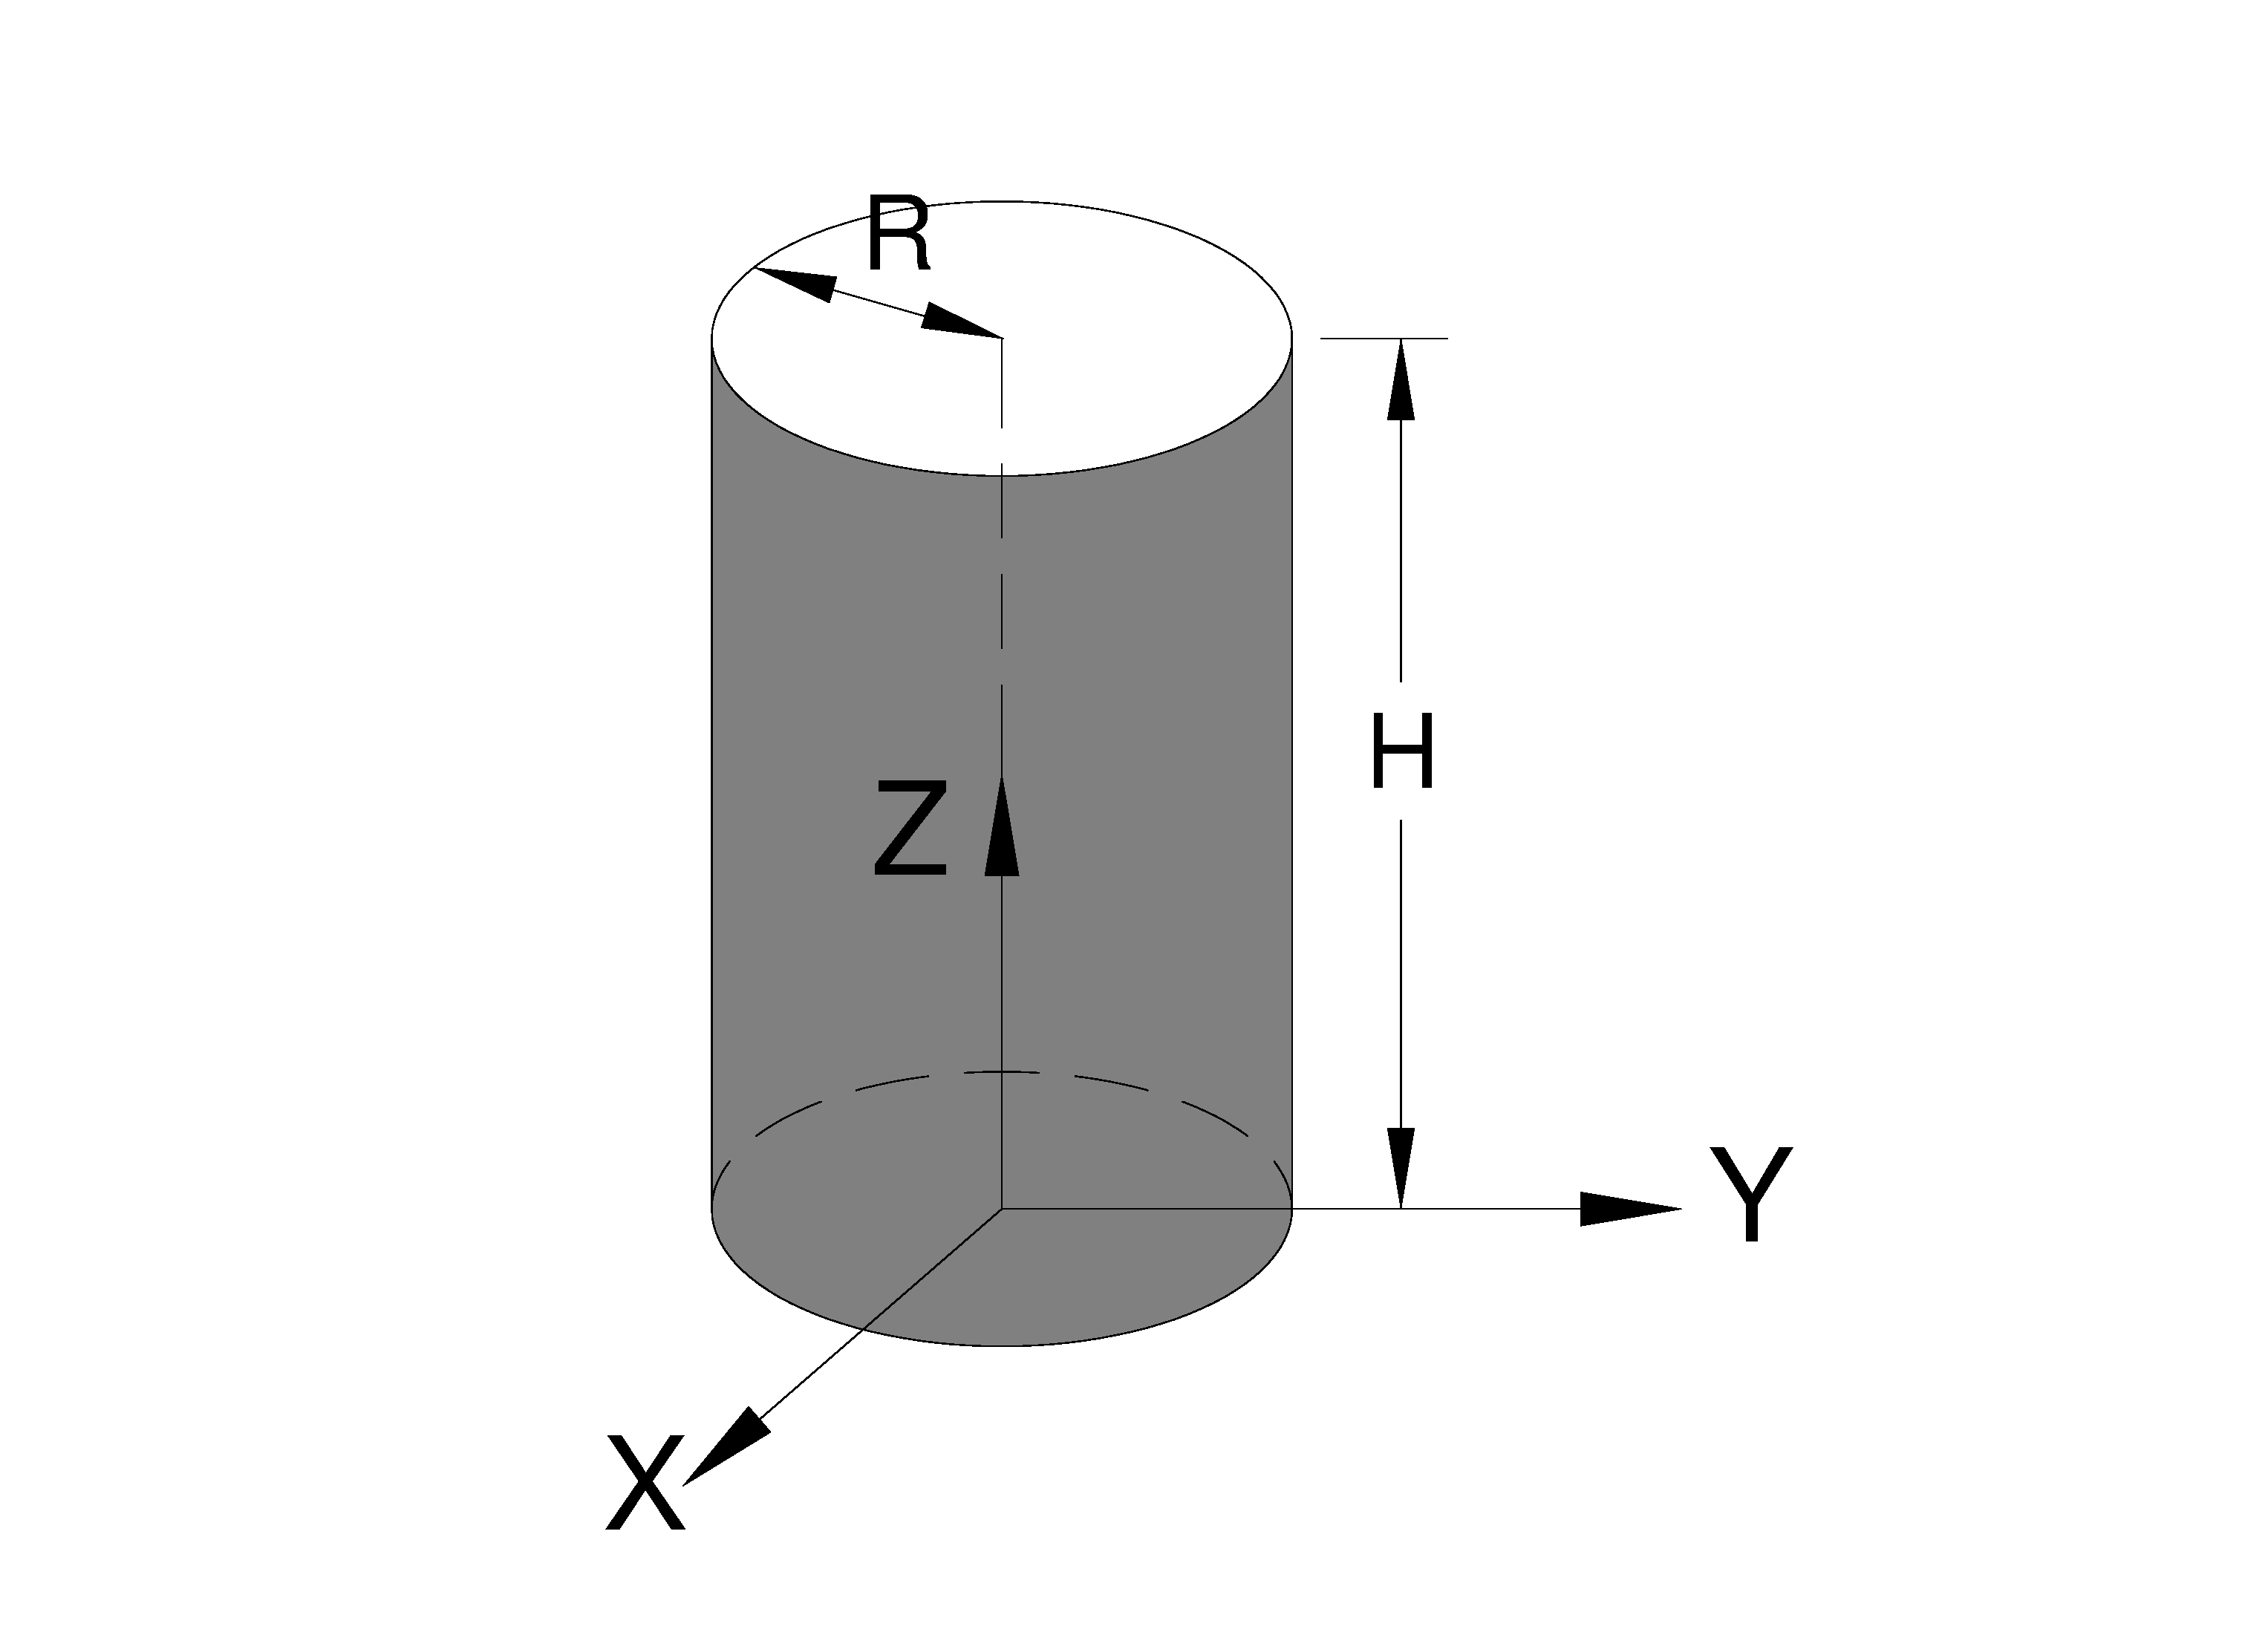
\includegraphics[height=6cm]{barracolgada.pdf} \label{figure1}
	\caption{Barra colgada}
	\label{BarraColgada}
\end{figure}
%
\begin{enumerate}

\item Esboce la configuracióon deformada de la barra.	

\item Calcule el tensor de deformaciones y descompóngalo en su componente 
simétrica: $[\varepsilon]$ y asimétrica  $[\omega]$

\item Cuáles son los valores máximos y mínimos de las deformaciones axiales, 
$\varepsilon_{xx}$, $\varepsilon_{yy}$, $\varepsilon_{zz}$, y en que puntos se 
presentan.

\item Cuáles son los valores máximos y mínimos de los desplazamientos: $u$, 
$v$, $w$ y en que puntos se presentan.

\item ¿Existen puntos exentos de rotación de cuerpo rígido?, responda sí o no y 
justifique su respuesta.
	
\item ¿Es posible encontrar puntos sometidos a distorsión angular?, 
responda sí o no y justifique su respuesta.
\end{enumerate}


\item  \label{punto05_d}  En la figura \cref{VigaMomentoflec} se muestra un 
medio continuo de sección rectangular de ancho unitario, altura $H$, soportado 
en un extremo ($X = 0$), y sometido en su otro extremo ($X = L$) a la acci\'on 
de un momento flector $M$ alrededor del eje $Z$. Si el campo de desplazamientos 
en el sistema coordenado $XYZ$ está dado por:
\[u= -\dfrac{M}{EI} X Y\, ,  \hspace*{10mm}	
v = \dfrac{M}{2EI}(X^2+ \nu (Y^2-Z^2))\, ,  \hspace*{10mm}	
w = \dfrac{\nu M}{EI} Y Z\, ,  \]
donde $u,v,w$ son los desplazamientos asociados a los ejes $X,Y,Z$ 
respectivamente. $E$ y $\nu$ son constantes  (positivas) del material e $I$ es 
el momento de inercia alrededor del eje Z de la sección transversal.
\begin{figure}[H]
	\centering
	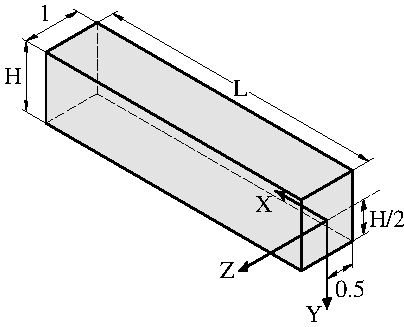
\includegraphics[height=6cm]{VigaMomento.pdf}
	\caption{Viga sometida a momento flector}
	 \label{VigaMomentoflec}
\end{figure}

\begin{enumerate}
\item En la figura \cref{ConfiguraFlector} se muestran esbozos de posibles 
configuraciones deformadas (sección achurada) de la viga mostrada en la figura 
\label{VigaMomento}. Determine en cada caso cual es la configuración correcta. 

\begin{enumerate}

\item[•] Para la sección transversal en $X = L$. 
\item[•] Para una sección longitudinal cuando $Y > 0$.
\item[•] Para una sección longitudinal asociada al plano ($Y = -H/2$)
\item[•] Para una sección longitudinal asociada al plano ($Z = 0$) 

\end{enumerate}

\begin{figure}[H]
	\centering
	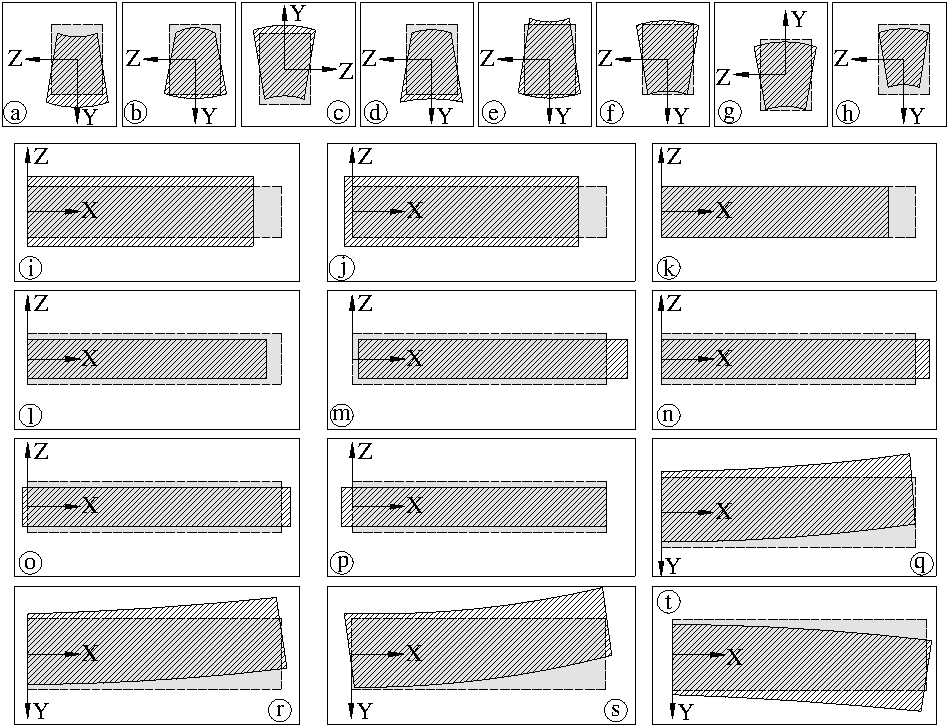
\includegraphics[height=12.00cm]{Configuracion.pdf}
	\caption{Posibles configuraciones deformadas de sección transversal}
	\label{ConfiguraFlector}
\end{figure}

\item Calcule el tensor de deformaciones  $[\varepsilon]$ y el de rotación 
$[\omega]$ 

\item Si el valor de la distorsión angular máxima es $\gamma$ = $\gamma_{\max}$ 
determine cual es el momento máximo posible, $M_{\max}$ que podría ser 
aplicado. 

\item¿Cuáles son las coordenadas $x,y,z$ de los puntos que experimentan 
mayores rotaciones de cuerpo rígido?

\item ¿Cuáles son los puntos que experimentan la menor rotación de cuerpo 
rígido? 

\item Cuales son los valores máximos y mínimos de las deformaciones axiales, 
$\varepsilon_{xx}$, $\varepsilon_{yx}$, $\varepsilon_{zz}$ y en que puntos se 
presentan.

\item ¿Cuáles son los valores máximos y mínimos de los desplazamientos, $u$, 
$v$, $w$, y en qué puntos se presentan?

\item ¿Existen puntos exentos de rotación de cuerpo rígido?, responda sí 
o no y justifique su respuesta.

\item ¿Es posible encontrar puntos sometidos a distorsión angular?, responda 
sí o no y justifique su respuesta.

\end{enumerate}

\item \label{punto07_d}  En la figura \cref{Solucion_Flamant} se  muestra la 
solución de un semi-espacio sometido a una carga lineal superficial $P$.  Los 
desplazamientos al interior del suelo debidos a la carga $P$ están dados por:
\begin{align*}
&u_r (r,\theta) = -\dfrac{2P}{\pi E} \ln{r} \cos \theta -\dfrac{(1 - 
\nu)P}{\pi E} \theta\, \sin\theta + B \cos \theta \\
&u_{\theta}(r,\theta) = \dfrac{2 \nu P}{\pi E} \sin\theta + 
\dfrac{2P}{\pi E}\ln{r}\sin\theta - \dfrac{(1 - \nu)P} {\pi E} 
\theta \cos\theta + \dfrac{(1 - \nu)P}{\pi E} \sin\theta - B \sin\theta\\
& w (r,\theta) = 0
\end{align*}
donde $E$ es el módulo de elasticidad,  $\nu$ es la relación de 
Poisson del material y $B$ es una constante positiva.
\begin{figure}[H]
	\centering
		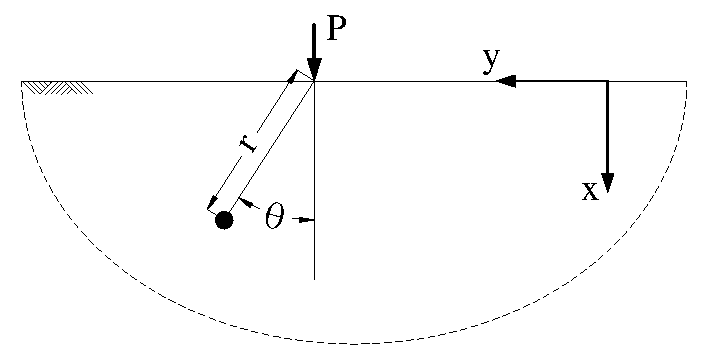
\includegraphics[height=3.0cm]{Flamat.pdf} 
		\caption{Soluci\'on carga vertical}
		\label{Solucion_Flamant}
\end{figure}

Si en un suelo sometido a la acción de dos estructuras que le transmiten  una 
carga lineal superficial, $P$ y $3P$, respectivamente tal como se muestra en la 
figura  \cref{figure3} se desea instalar una tubería, perpendicular al plano 
mostrado ($XY$), de diámetro despreciable, en el punto indicado  en la figura 
\cref{figure3}.
\begin{figure}[H]
	\centering
	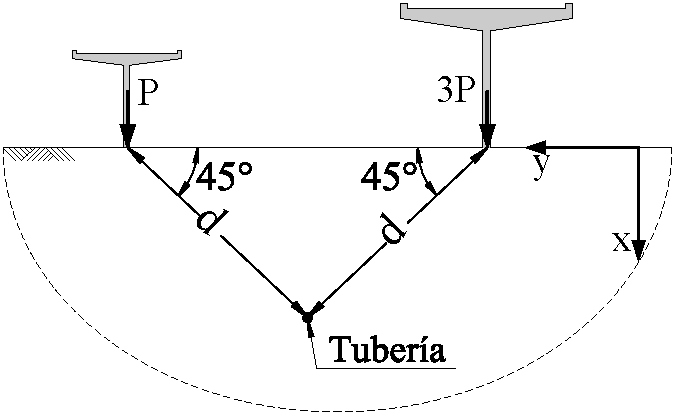
\includegraphics[height=3.5cm]{ProblemTub.pdf} 
	\caption{Estructuras y tubería.}
	\label{figure3}
\end{figure} 

\begin{enumerate}
\item Determine cuál es el valor de la deformación axial máxima.

\item  Si la máxima deformación angular a la que puede ser sometida la 
tubería sin fallar, es igual a: $\gamma_{\max}$. ¿Cuál es el máximo valor 
de la carga distribuida $P$ que pueden transmitir las estructuras para que 
la tubería no falle?

\item Esboce la configuración deformada de la partícula correspondiente al 
punto donde se ubica la tubería. Solo considere el plano $xy$. 
\end{enumerate}


\item \label{punto08_d} En la figura \cref{BarraApoya} se muestra una barra de 
radio $R$ y longitud $L$. El campo de desplazamientos   en el sistema 
coordenado $xyz$, está dado por:
\[u= -\theta yz\, , \hspace{15mm} v= \theta xz\, , \hspace{15mm} w= 0\, .\]
donde $u,v,w$ son los desplazamientos asociados a los ejes $x,y,z$ 
respectivamente. $\theta$ es una constante positiva.
\begin{figure}[H]
	\centering
	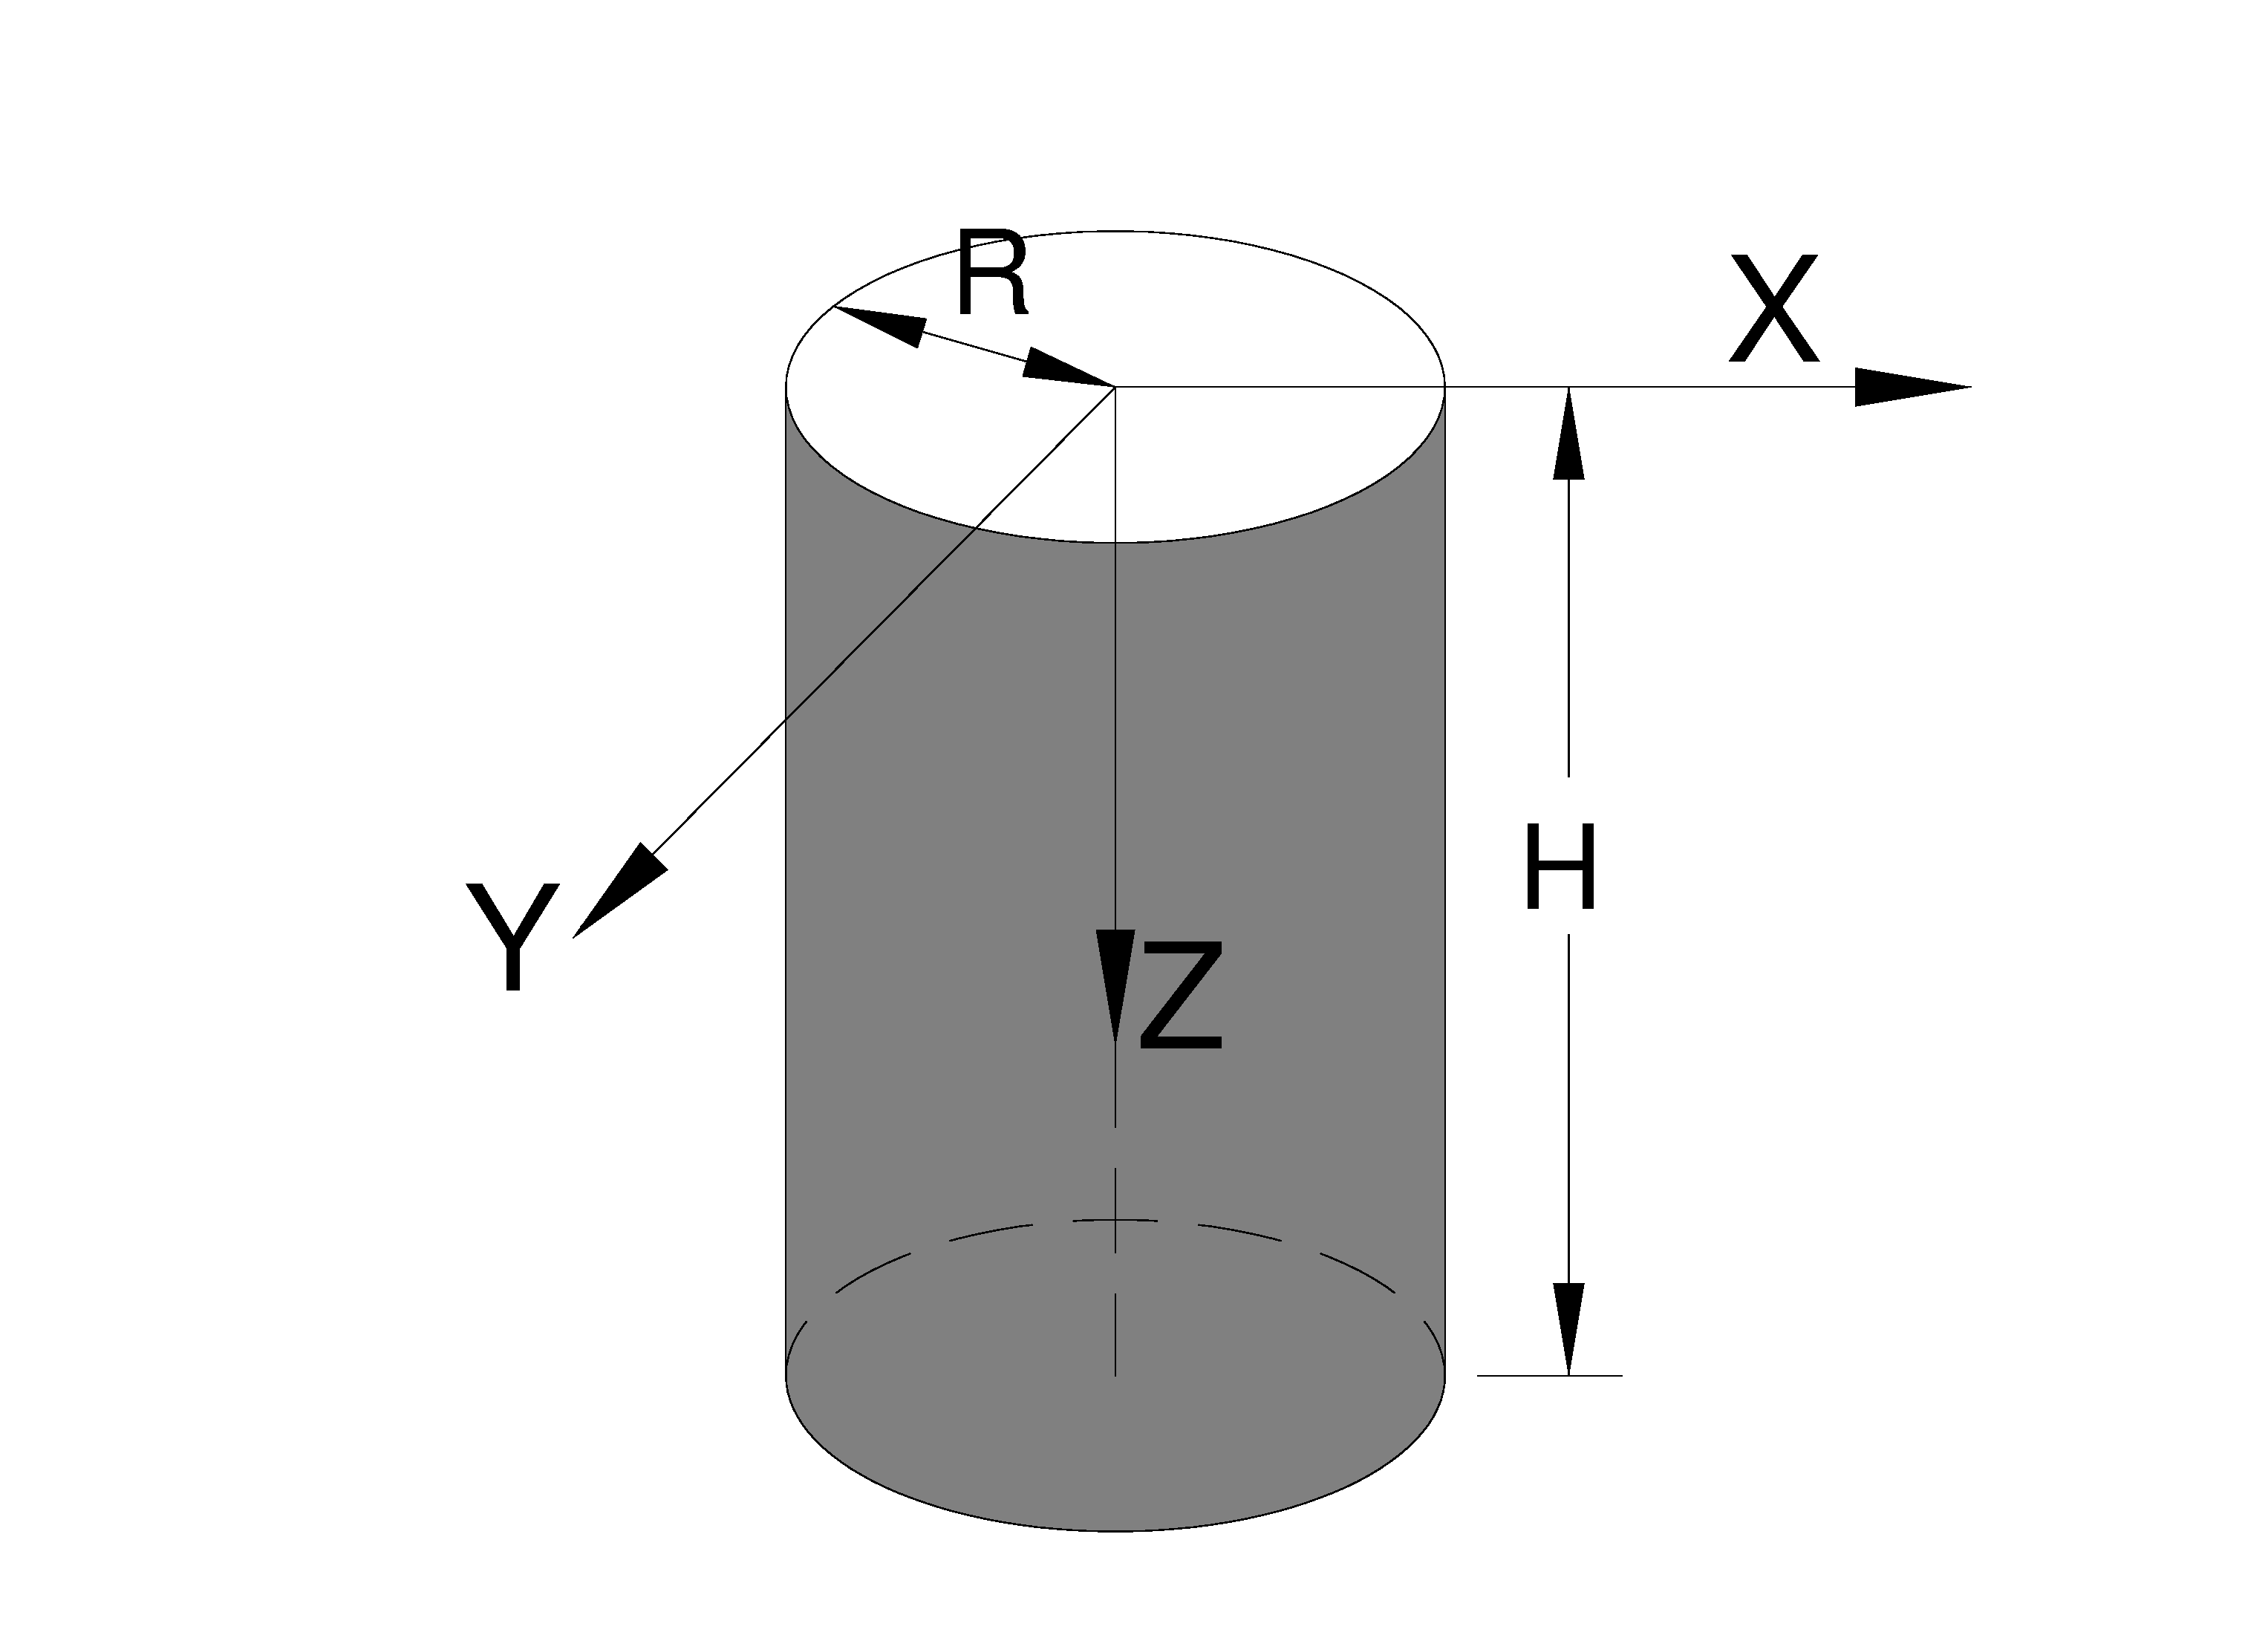
\includegraphics[height=5cm]{barraapoyada.pdf} 
	\caption{Medio Continuo}
	\label{BarraApoya}
\end{figure}

\begin{enumerate}
\item Dibuje la configuración deformada de la barra. 
\item Calcule el tensor de deformaciones, $[D]$, y determine: tensor de 
deformación $[\varepsilon]$ (simétrico) y tensor de rotación $[\omega]$ 
(asimétrico).
\item Ilustre la deformación de la partícula en el punto de coordenadas $y = R$ 
y $x = 0$. Para la ilustración use cuadrados de tamaño diferencial contenidos 
en los planos $xy$, $xz$, $yz$ de forma independiente. En la ilustración debe 
incluirse los efectos de cuerpo rígido.
\item ¿Cuáles son los puntos que experimentan mayores rotaciones de cuerpo 
rígido?
\item ¿Cuáles son los valores máximos y mínimos de los desplazamientos, $u$, 
$v$, $w$ y en que puntos se presentan:
\item  ¿Es posible encontrar puntos sometidos a distorsión 
angular?, responda sí o no y justifique su respuesta.
\end{enumerate}

\item  \label{punto09_d} En la figura \cref{cuna} se presenta una cuña de 
espesor $t$ sometida a la acción de una carga (en el plano $XY$) distribuida 
sobre su perímetro.
%
\begin{figure}[H]
	\centering
	{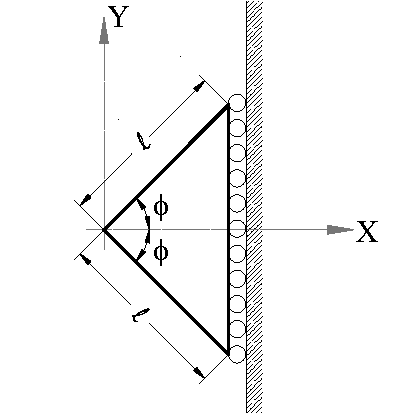
\includegraphics[width=7cm]{Cunasup.pdf}}\
	\hspace{2 cm}
	\caption{Cuña de espesor $t$}
	\label{cuna}
\end{figure}
%
El campo de desplazamientos de la cuña  esta dado por:
\[u(x,y) = \dfrac{2B}{E} (\cot \phi + \nu \tan \phi) (x - l\cos \phi)\, ,
\hspace{8mm}  v(x,y) = - \dfrac{2B}{E} (\tan \phi + \nu \cot \phi) y\, ,\]
donde $B$, $E$ y $\nu$ son constantes positivas.

Además, se sabe que:
\[ \sigma_{xx} = \dfrac{E}{(1 - \nu^2)} (\varepsilon_{xx} + \nu 
\varepsilon_{yy})\, ,\hspace{5mm}
\sigma_{yy} = \dfrac{E}{(1 - \nu^2)} (\varepsilon_{yy} + \nu \varepsilon_{xx}) 
\hspace{5mm}\, ,
\tau_{xy} = \dfrac{E}{2(1 + \nu)} \gamma_{xy}\, .\]

\begin{enumerate}
\item Dibuje la configuración deformada de la cuña. 

\item Ilustre la deformación de la partícula en el punto de coordenadas $X 
= 0$ y $Y = 0$. En la ilustración deben incluirse los efectos de cuerpo 
rígido. 	

\item Si $\nu=0.25$ y $\phi=53.13^{\circ}$, determine la reacciones (Fuerzas) 
en el soporte .
\end{enumerate}

\item  \label{punto10_d} Si el campo de desplazamientos para la barra mostrada 
en la \ref{def:Mario} está dado por:
\[u\left( x \right) = -\dfrac{1-\nu^2}{E} \sigma_0 x\, ,\quad v=0\, ,\quad 
w\left( z \right) = \nu \dfrac{1+\nu}{E} \sigma_0 z\, .\]
\begin{figure}[H]
	\centering
	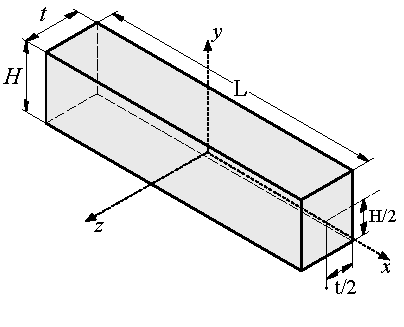
\includegraphics[height=5cm]{Viga.pdf} 
	\caption{Viga de Longitud $= L$, Altura $=H$ y Espesor $=t$. El origen del sistema coordenado coincidiendo con el centroide de la barra.}
	\label{def:Mario}
\end{figure}

\begin{enumerate}
\item Explique a que acciones externas está sometida la barra.

\item Dibuje la configuración deformada de la barra.

\item \textquestiondown Hay partículas sometidas a rotaciones de cuerpo 
rígido? (responda sí o no y justifique su respuesta).

\item \textquestiondown Hay partículas que {\textbf{NO}} experimenten 
distorsiones angulares? (responda sí o no y justifique su respuesta).

\item En que coordenadas está la partícula que sufre mayor deformación 
axial y cuál es el valor de esta deformación.

\item En que coordenadas está la partícula que sufre mayor distorsión 
angular y cuál es el valor de esta deformación.

\item Encuentre los desplazamientos y deformaciones del punto de 
coordenadas $(0,0,0)$.
\end{enumerate}

%
% ***** Empieza modelos constitutivos
\item   \label{punto11_d} Para un campo de desplazamientos dado por:
\[\mathbf{u} = a(x^2 - 5y^2)\hat{\imath} + (2ax y)\hat{\jmath} \]

\begin{enumerate}
\item Determinar el tensor de deformaci\'on;
\item Obtener las deformaciones principales.
\end{enumerate}

\item \label{punto12_d} En la figura \cref{fig:barra} se presenta una barra 
sobre la cual se aplica una fuerza en dirección $x$ $F_{x}$, que genera  un 
esfuerzo constante $\sigma_x$ sobre la sección transversal donde está aplicada. 
La barra inicialmente está  separada de una lámina delgada de acero una 
distancia $d$ tal y como se muestra en \cref{sfig:barra2D}. El campo de 
desplazamientos para la barra mostrada está dado por:
\[u\left( x \right) = \dfrac{1}{E_1}  x \sigma_x, \hspace{10mm} v=0\, , 
\hspace{10mm}
w\left( z \right) = - \dfrac{1}{E_2}  z (H^2 - y^2) \sigma_x\, ,\]
donde $E_1 = 200000 \text{ kgf/cm}^2$,   y $E_2 = 1000000 \text{ kgf/cm}^4$, $L 
= 1000 \text{ cm}$, $H = 10 \text{ cm}$. $\sigma_x$ es el esfuerzo en dirección 
$x$ el cual tiene una variación en el tiempo de acuerdo a como lo muestra la  
\cref{sfig:stress}.  

\begin{figure}[H]
	\centering
	\subfloat [Configuración inicial de la barra en 3D. Aplicación de la 
	fuerza]{ 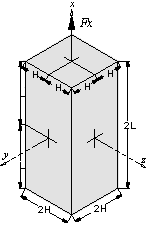
\includegraphics[width=1.6in]{Barra.pdf}\label{sfig:barra3D}}
	\hspace{0.7cm}
	\subfloat [Vista plano $xz$. Separación inicial barra - lámina, d = 2.0 cm. 
	$\phi = 45^\circ$.]{ 
	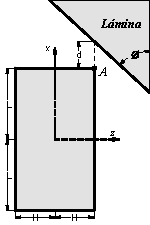
\includegraphics[width=1.6in]{BarraPared.pdf}\label{sfig:barra2D}}
	\hspace{0.7cm}
	\subfloat [Curva de esfuerzo.]{ 
	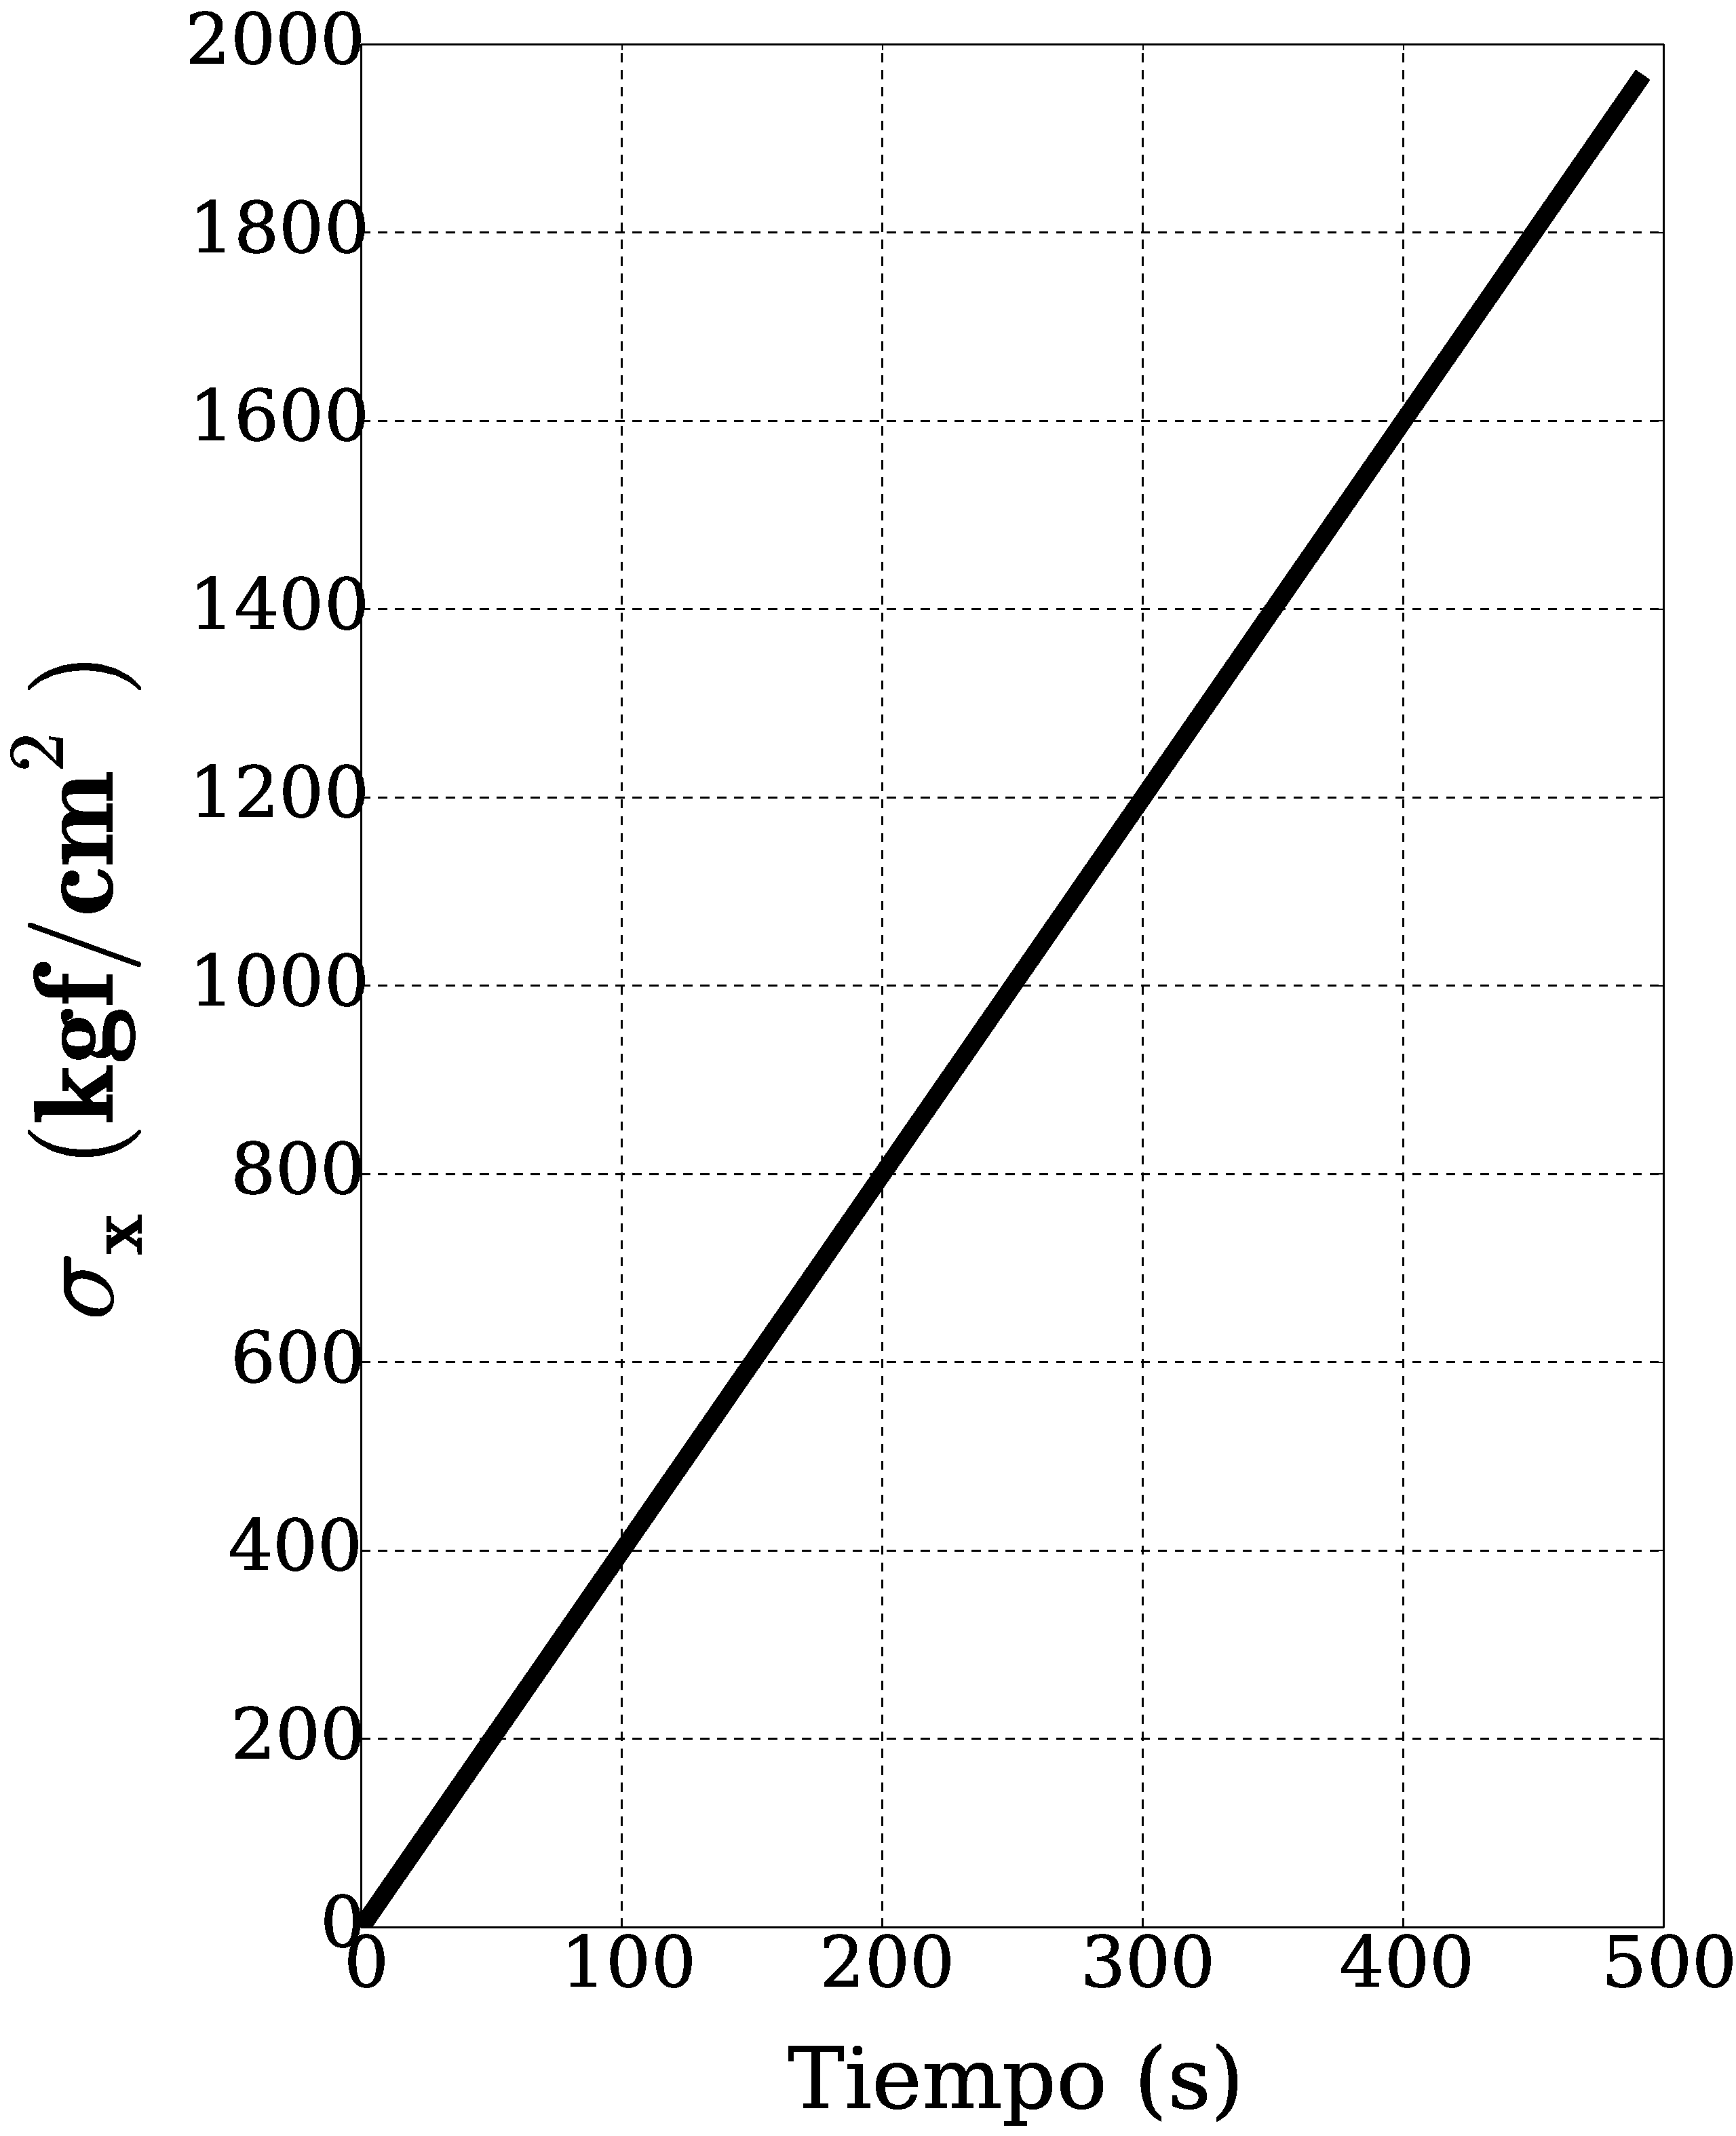
\includegraphics[width=1.9in]{CurvaEsf.pdf}\label{sfig:stress}}			
    \caption{Barra sometida a fuerza axial $F_{x}$}
	\label{fig:barra}
\end{figure}


\begin{enumerate}
\item Para el punto A de la barra con coordenadas  $(x,y,z) = (L, 0, B)$ 
grafique los desplazamientos $u$ y $w$ en función de tiempo. 

\item Dibuje la configuración deformada de la partícula para el punto de 
coordenadas $(x,y,z)=$ $(0,0,0)$ 

\item  Si el valor de $\sigma_x = 50 \text{ kgf/cm}^2$ y se estudian solo 
los puntos de la cara $ z = 1.0 cm$ determinar el valor de la distorsión 
angular máxima y las coordenadas $x,y,z$ de los puntos  en que se 
presenta. 
	
\item Si el esfuerzo  $\sigma_x$ se incrementa  hasta que el punto  $A$ con 
coordenadas  $(x,y,z) = (L, 0, B)$ toque la lámina, determine el tiempo $t$  en 
el que la barra toca la lámina. ¿Cuáles serían las coordenadas finales $x$, $z$ 
del punto A en ese instante?
\end{enumerate}


\item  \label{punto13_d}  En un ensayo de un elemento de concreto se mide la 
deformación en un mismo punto mediante tres galgas de deformación. Las galgas 
de deformación se disponen en un arreglo tal y como se muestra en la 
\cref{ensayogalga}.
\begin{figure}[H]
	\centering
	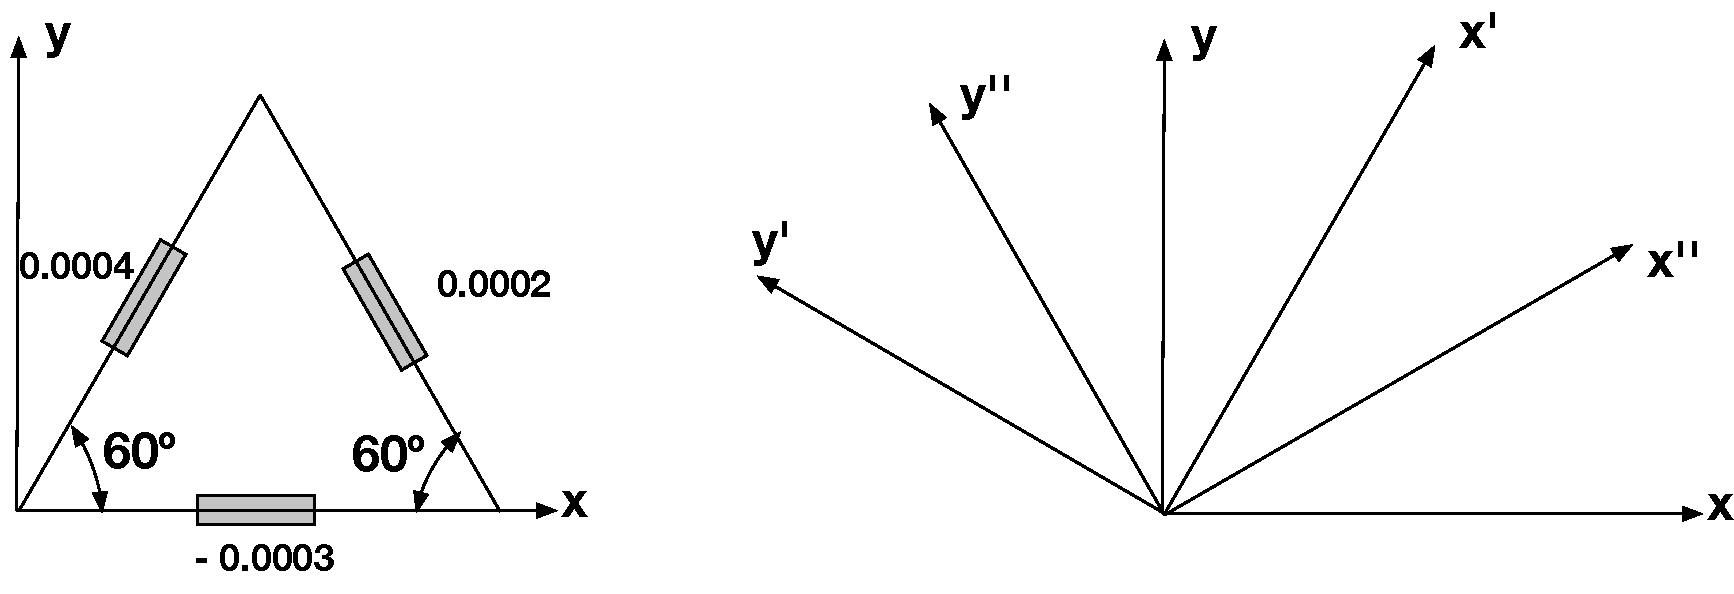
\includegraphics[width=4.5in]{galgas.pdf}
	\caption{Galgas de deformación}
	\label{ensayogalga}
\end{figure}


Si las galgas solo registran la deformación axial y las mediciones de laboratorio reportaron: $\varepsilon_{xx} = -0.0003$; $\varepsilon_{x'x'} = 0.0004$; $\varepsilon_{y''y''} = 0.0002$. Se solicita

\begin{enumerate}
\item Tensor de deformaciones en el sistema $xy$, $x'y'$ y $x''y''$. 

\item Distorsión angular máxima. 

\item Deformación axial máxima.

\item Configuración deformada de la partícula.
\end{enumerate}

\end{enumerate}

\end{document}
